\documentclass[a4paper]{article}

%% Language and font encodings
\usepackage[T1]{fontenc}
\usepackage[utf8x]{inputenc}
\usepackage[english]{babel}

\usepackage[colorlinks=true, allcolors=blue]{hyperref}

\urlstyle{tt}
\newcommand{\email}[1]{\href{mailto:#1}{\tt{\nolinkurl{#1}}}}
\newcommand{\orcid}[1]{ORCID: \href{https://orcid.org/#1}{\tt{\nolinkurl{#1}}}}

\usepackage[sfdefault,lf]{carlito}
%% The 'lf' option for lining figures
%% The 'sfdefault' option to make the base font sans serif
\usepackage[parfill]{parskip}
\renewcommand*\oldstylenums[1]{\carlitoOsF #1}
\usepackage{fancyhdr}
\usepackage{natbib}
\usepackage{authblk}
\usepackage{amssymb}
\usepackage{algorithm,algpseudocode}
\usepackage{graphicx}

\usepackage{tikz}
\usetikzlibrary{shapes}


\RequirePackage{ifthen}
\usepackage{latexsym}
\RequirePackage{amsmath}
\RequirePackage{amsthm}
\RequirePackage{amssymb}
\RequirePackage{xspace}
\RequirePackage{graphics}
\usepackage{graphicx}
\usepackage{caption}
\usepackage{subcaption}
\usepackage{xcolor}

\setlength{\headheight}{41pt}

%% Sets page size and margins
\usepackage[a4paper,top=3cm,bottom=2cm,left=3cm,right=3cm,marginparwidth=1.75cm]{geometry}

%% Useful packages
\usepackage{amsmath}
\usepackage{graphicx}
\usepackage{booktabs}
\usepackage{subcaption}

\usepackage{keyval}
%\usepackage{listings}
\usepackage{xspace}
\usepackage{mathrsfs,paralist, amsmath,amssymb,url,listings,mathrsfs}
\usepackage[colorinlistoftodos]{todonotes}
\usepackage{framed}
\usepackage{lipsum}




%\renewcommand{\headrulewidth}{0pt}
\pagestyle{plain}
\title{Learning to Generate Game Content Without Human Supervision }
\author[1]{Adam Summerville}

\begin{document}
\maketitle
\thispagestyle{fancy}

\section{Introduction}

PCG has been a part of computer games for the majority of their existence (Beneath Apple Manor - 1978).  For most of this time, generation has required human designers to encode all of the rules governing the generation (achieved through many different formalisms: imperative code, declarative code, grammars, evolutionary geno/phenotypes, fitness criterions, search).  This is a difficult endeavor for a number of reasons:

\begin{enumerate}
\item For a designer in process, design decisions are rarely accurately accessible via introspection **CITE STUFF HERE**
\item Performing a critical deep dive into a piece of work to access the design decisions is not something done lightly, making up entire fields of study (e.g. Digital Humanities)
\item Formalizing all design decisions is difficult, as humans often have hidden biases / foreseeing all possible outcomes of an algorithm is impossible in general (see decidability) and is difficult in specific (see the fields of automated testing/code verification)
\end{enumerate}

This is not to say that it can not be done, as, obviously, people have done this.  But it is to say that in general it is a hard, arduous endeavor that can still lead to feelings of ``oatmealishness'' (** CITE KATE and MIKE), i.e. content that while different in countless different ways, still feels the same.  

However, the design decisions to generate a piece of content do not need to be exhaustively encoded, they can be learned.  The design of an artifact is latent within the artifact itself.  The goal of this work is to learn that latent design, so as to be able to generate perceptually similar artifacts, and to do so from observation, with minimal human supervision.

Towards this end, I propose three related systems, each one possible of working in isolation, but intended to work together:

\begin{itemize}
\item \textit{Nayru} - Given access to a game - extract all of the content from it, the levels, the behaviors, the interactions, etc.
\item \textit{Farore} - Given descriptions of game entities (e.g. their behaviors) - generate new entities that are *most importantly* sound, and that have similar properties to existing entities
\item \textit{Din} - Given a set of game levels - generate new levels with similar perceptual properties

\end{itemize}

These three systems (named after the goddesses from \textit{The Legend of Zelda} series) are intended to work with minimal human supervision (the only thing a human need provide is a game) and while they can work in isolation (a designer could feed \textit{Din} levels without every worrying about \textit{Nayru}) they are intended to work such that \textit{Nayru} provides the necessary input for \textit{Farore} and \textit{Din}.  

These three (hereafter referred to as \textit{Hylia} when discussing the system as a whole) are intended to resolve a number of research questions:

\textbf{Question 1: How can a machine learn the important mechanical properties of the content?}

Currently, techniques such as Generative Adversarial Networks (GANs) or Variational AutoEncoders (VAEs) are popular techniques for image generation.  Certainly, it would be possible to supply images of game levels (these exist in abundance on the internet **CITE VGATLAS**), but visual signifiers are only one portion of the semiotics of a game.  The mechanical properties of the game entities are at least equally as important (and certainly visuals can deceive, as two visually identical entities might have different properties).  While image based techniques might be able to generate visually acceptable levels, without a way of encoding these properties they are going to lack the expressivity of a generator which has access to such properties.  Previous machine learned approaches have either operated on the visual level or with designer specified mechanical properties.   I aim to answer the question of how to learn the mechanical properties in a way that enables down stream use (e.g. for use in \textit{Din}).


\textbf{Question 2: How should content be represented such that it can be efficiently learned for generation?}

Most uses of machine learned generation have focused on two types of data: text and images.  Both have standard structures and associated machine learning techniques (e.g. text as a sequence handled by Long Short-Term Memory Recurrent Neural Networks and images as RGB Tensors handled via GANs or VAEs).  Game levels have some features similar to both, but are often composed of multiple pieces of arbitrary shape and size.  Behaviors have no commonly agreed upon format.  I aim to answer the question of how to best represent game content for the sake of efficient training and generation.

\textbf{Question 3: How do we assess whether a learned generator has learned to generate the desired content?}

Evaluation of PCG for games has largely focused on examining a few hand-picked generated artifacts or on visually analyzing a histogram of the expressive range of a generator.  The former is prone to cherry picking, leaving one to wonder what the expressive capabilities of the system actually are, while the latter is rarely tied back to an intuitive understanding (e.g. Is it good or bad to have a wide histogram? What does it mean for certain portions of the space to be under or over represented? Are the dimensions shown actually worthwhile?).  For a classical PCG system these evaluations are perhaps unsatisfying, but given that authors do not necessarily make any claims about the generative space of the systems, they are not mission-critical.  On the other hand, machine learned PCG systems make the claim that they are accurately learning the design space of the original training data, so it is necessary to show that the generators are able to generate similar content while not memorizing the training data.




The primary contributions of this research are two-fold:
\begin{enumerate}
\item The development of techniques to learn the properties of game content automatically from observation
\item The development of formalisms for representing rules, entities, and levels in a manner amenable to the training of machine learning systems and then generating new content that is similar
\item The development of techniques for evaluating machine learned generators
\end{enumerate}


Which represent contributions to the fields of machine learning, procedural content generation, and automated game design research.


There are three components to \textit{Hylia}:

\begin{itemize}
\item Learning behaviors and levels from observation
\item Generating behaviors
\item Generating levels
\end{itemize}

so it is important to place these components in context with existing work.



\subsection{Learning From Observation}

Learning a representation of a black-box system is a problem that has been approached before.  Depending on the desired properties of the representation and the observed properties of the system, different approaches are suitable.  For deterministic discrete state-space system there exists a body of work to learn Finite State Machines from observation.  

Learnlib \cite{Introduction to Active Automata Learning from
a Practical Perspective?} is a library that learns Mealy machines via active learning.  A Mealy machine is a deterministic finite automata that differentiates input and output alphabets. The active learning process iterates between exploration and testing phases.  In the exploration phase, a sequence of system inputs are entered and the states reached are observed.  In the testing phase, the hypothesized system is compared to the actual system and divergence in behavior is tracked so as to provide an input sequence for the next exploration phase.

For systems that have a mixture of real valued behaviors (e.g. position changing in real time) that change depending on discrete modes (e.g. an aircraft maneuvers differently while turning than it does while traveling at a constant heading) Hybrid Automata (HA) represent a natural formalism. 
Given the desirable properties of HAs, and the ready availability of tools for dealing with them, many researchers have explored automatically recovering these high-level models from real-world system behaviors.
CHARDA shares motivations with HyBUTLA~\cite{niggemann2012learning}, which also aimed to learn a complete automaton from observational data.
%% A superficial difference is that their work operates on multiple episodes of observations; CHARDA could easily be extended in that way.
%% MM: I'd delete the above sentence. Since it's a superficial distinction it's only a distraction. 
%% Joe: OK
HyBUTLA seems able to learn only acyclic hybrid automata, since it works by constructing a prefix acceptor tree of the modes for each observation episode and then merges compatible modes from the bottom up.
%% MM: added "for each observation episode" above since I'm suggesting deleting the previous sentence.  
%% Joe: OK
Moreover, HyBUTLA assumes that the segmentation is given in advance and that all transitions happen due to individual discrete events, presumably from a relatively small set.


Santana \textit{et al.}~\cite{hybridmodels2015santana} learned Probabilistic Hybrid Automata (PHA) from observation using Expectation-Maximization.  At each stage of the EM algorithm a Support Vector Machine was trained to predict the probability of transitioning to a new mode. Their work requires a priori knowledge about the number of modes.


Ly and Lipson used Evolutionary Computation (EC) to perform symbolic regression \cite{Learning Symbolic Representations of Hybrid Dynamical Systems} to find common behaviors across different modes, as well as to find guard transitions between modes.  Adding more parameters in the symbolic regression step will always increase model accuracy, so they used the Akaike Information Criterion (AIC) to balance model accuracy with model complexity.  This work makes minimal assumptions about the types of behaviors that can be found in a given mode, but does require a priori knowledge about the number of modes that will be found in the dataset. Moreover, since their work assigns individual datapoints, not intervals, to a mode, their approach can only model stationary processes.

Other work has sought to learn non-HA descriptions of dynamical systems' behavior. 
Several approaches have sought to learn models that describe dynamical systems' behavior.
Hidden Markov Models~\cite{baum1966statistical} learn probabilistic state transitions between a hidden state and the observed data.
The Infinite HMM ~\cite{beal2002infinite} extends this to an unbounded number of states which assumes a Chinese Restaurant Process governs the state space.
These approaches do not characterize guard \textit{conditions}, but instead learn the \textit{probability} of taking state transitions at each instant. 
Some techniques have leveraged certain inductive biases from biological or other domains to obtain good results.
Kukreja \textit{et al.}\cite{kukreja2005least} found models of switched mode systems given prior knowledge about the locations of the switchpoints, and Bridewell \textit{et al.}\cite{bridewell2008inductive} used exhaustive search over model structures to best explain observed data without assuming fixed switchpoints.

In the games domain, there has been minimal work in learning games from observation. In  \cite{bjornsson2012learning}, an approach was introduced for learning the rules of a simple game through observation. This approach includes learning a \textit{DFA} (\textit{deterministic finite automata}) as a model for game rules. Their work focused on learning the rules of a board game and is tied to this domain.  In fact a large portion of the work relies not just on observing moves that took place but being given all of the moves that could have taken place.

\subsection{Procedural Content Generation}


The procedural generation of level content has been popular in commercial, hobbyist, and academic circles with recent years seeing increasing amounts of interest in procedural generation.   A game jam devoted to procedural content, PROCJAM, had 99 games submitted in 2015 and nearly double, 173, in 2016 \cite{PROCJAM2015,PROCJAM2016}.  While PCG has focused on a number of different game aspects such as characters \cite{SOMETHING}, narrative \cite{SOMETHING}, levels have been a major area of focus.   

\subsubsection{Level Generation - Human Design Approaches}
Platformer levels have represented one of the most fecund areas of research, particularly levels for \textit{Super Mario Bros.}  As the progenitor of the platformer genre, as well as one of the most popular games of all time, \textit{SMB} has been the most common game for level generation.  A large number of different approaches have been taken for \textit{SMB} level generation.

Many approaches have utilized hand authored level pieces and rule systems to generate levels. The Probabilistic Multi-Pass (ProMP) generator by Ben Weber \cite{mario2010} creates a base level and then iterates through it adding new components on each pass.  Components have a probability for being added, but the probabilities are tuned based on other constraints (e.g. if the maximum number of gaps has been reached, the probability for a new gap is set to 0).  The Occupancy-Regulated Extension (ORE) approach of Mawhorter \cite{mawhorterORE} places hand-authored pieces to generate whole levels.  Each piece was annotated with anchor points which represent places where other pieces may be placed.   The system by Baumgarten \cite{mario2010} uses linear discriminant analysis to provide a low-dimensional embedding of player skill and then uses that value to determine which hand-crafted level pieces to place to generate a complete level. 

Hopper by Takahashi and Smith \cite{mario2010} attempts to generate levels that imitate the style of \textit{Super Mario World}.  Hopper uses rules to probabilistically place pieces, the weights of which are manually tuned based on inferred player type and skill level. Tanagra \cite{tanagra} is only Mario adjacent, creating levels for a platformer with similar components to that of Super Mario.  Tanagra uses a rhythm-based framework to generate ``beats'' of player action in varying rhythms.  These beats may take the form of gaps the player must jump over or an enemy the player must defeat.   Tanagra uses reactive planning to choose beats, create the corresponding level segments, react to user input, and generate playability constraints.  The playability constraints are then solved in a second pass by a constraint solver which attempts to prevent unplayable levels from being created.  Tanagra can work solely as a generator, or it can work in conjunction with a human designer as a co-creative assistant.  The human can design level segments which Tanagra will incorporate in its generation, or the human can author at a more abstract beat level which Tanagra can then reify.

The approach of Shimizu and Hashiyama \cite{mario2010} utilized offline interactive evolutionary computation to generate candidate level pieces and then placed those based on player modeling that attempted to classify how likely players were to break blocks, collect coins, and defeat enemies.  The approach of Sorenson and Pasquier \cite{sorpasq} uses evolutionary computation with an objective that rewards alternating periods of high and low challenge, with the goal of keeping player's engaged but not overwhelmed.  

While Mario-like platformers have been the dominant testbed for procedural level generation, there has been some interest in generating ``dungeons'' for games like \textit{The Legend of Zelda}.  While platformers are 2 dimensional games viewed from the side, Zelda-likes have a top-down perspective and the player generally has much more freedom to explore the entirety of the level.

  The system of Valls-Vargas, et al. \cite{VARGASPLOTPOINTS} performs an exhaustive breadth-first search to find all possible  mission spaces for an input set of plot points.  Once all possible missions have been constructed, they are evaluated for fitness based on how closely the mission matches the desired properties set forth by the designer.  This approach will find the best solution, as defined by the evaluation criteria, but can only handle missions of a limited size due to the exhaustive nature of the search.  

Grammar based methods are not guaranteed to find an optimal solution, but their limited expansion rules direct the search to more desirable regions of the possibility space much more efficiently than an breadth first search.  Joris Dormans's system \cite{JDADVENTURE} uses grammars for both the mission and level spaces.  The mission space is constructed 
by a graph grammar where nodes in the graph make up player actions such as "Defeat Boss" or "Unlock Door".  From a starting seed, production rules are applied pseudo-randomly until all non-terminal nodes have been converted to terminal nodes.Once the mission space of the level has been constructed, a shape grammar is applied on the mission graph.  The first node of the mission graph is taken and the system looks for a shape grammar rule that satisfies the mission node symbol, finds a location where the rule could be applied and applies it. A similar grammar based system was developed by van der Linden, et al. \cite{VDLPROCGENLEVEL}  that uses grammars for both mission and level generation as well.  The advantage to van der Linden's work is that multiple mission actions can occur at the same location, e.g. kill a dragon and get dragon's treasure could both occur at the same location.  The grammar based methods have the advantage of being intuitive, but unless the grammar is heavily constrained it can be hard to guarantee that the levels produced match designer criteria while retaining uniqueness.  

Genetic algorithm solutions have the advantage of being able to find a wide range of optimal solutions; However, they come with no guarantees that the optima found are global or that they will terminate in any amount of time.  The key factors that determine the type of level created by a genetic system are the genotype and phenotype representations and the evaluation metric. The system developed by Sorenson and Pasquier \cite{SORPASLEVEL} has direct genotype to phenotype mapping as elements in the phenotype equate to the placement of elements in the level. Their evaluation metric seeks to keep interactions along the optimal path varied.  To keep genetic diversity while also ensuring the validity of produced levels, they used a Feasible-Infeasible Two-Population split.  By considering only the positioning of game elements, their system considers the mission space tangentially, by assuming that a good level space will lead to a good mission space. Valtchanov and Brown \cite{VALTCHANOVEVOLVE} 
created a system that uses a tree based genotype to handle room to room placement.  Their fitness evaluation rewards novelty and room interconnectedness, but only considers player experience by guaranteeing the maximum optimal path length.  Hartsook, et al. \cite{hartsook} used a similar tree based genome, but their fitness function considers the distance between critical nodes, 
length of sidepaths, average number of sidepaths per non-critical node, total 
number of sidepaths, total number of nodes, and environmental transitional probabilities.  

While the genetic algorithms can produce a variety of levels, they have no guarantees about content produced. At the opposite end of the spectrum are constraint based solvers that provably produce levels that meet the designer's desires. In these systems, the designer sets up a system of logical properties and relations and the solver finds solutions that match the designer's criteria.
Horswill and Foged \cite{HORSWILLCONSTRAINT} developed a constraint solver that uses constraint propagation to place items within a level to meet a desired player experience, but it requires a level annotated with the desired player path. 

The above approaches all rely on human design intuition at some level.  Some stitch together human-authored snippets (Baumgarten's, ORE, ProMP), while others use human authored rules to generate level geometry (Tanagra, Hopper), while others  utilize human design intuition to score evolved content ( Sorenson and Pasquier, Shimizu and Hashiyama), and some rely on human design intuition about playability (Horswill and Foget).  More recently there has been interest in generators that do not require humans to author at the rule or design level and instead utilize machine learning techniques to generate levels.

\subsubsection{Level Generation -Machine Learned Approaches}

Dahlskog et al. trained $n$-gram models on the levels of the original \textit{Super Mario Bros.} game, and used these models to generate new levels~\cite{dahlskog2014linear}. As $n$-gram models are fundamentally one-dimensional, these levels needed to be converted to strings in order for $n$-grams to be applicable. This was done through dividing the levels into vertical ``slices,'' where most slices recur many times throughout the level~\cite{dahlskog2013patterns}. This representational trick is dependent on there being a large amount of redundancy in the level design, something that is true in many games. Models were trained using various levels of $n$, and it was observed that while $n=0$ create essentially random structures and $n=1$ create barely playable levels, $n=2$ and $n=3$ create rather well-shaped levels.


In \cite{snodgrass2014experiments} Snodgrass and Onta{\~n}{\'o}n present an approach to level generation using multi-dimensional Markov chains (MdMCs) \cite{ching2007multi}. An MdMC differs from a standard Markov chain in that it allows for dependencies in multiple directions and from multiple states, whereas a standard Markov chain only allows for dependence on the previous state alone. In their work, Snodgrass and Onta{\~n}{\'o}n represent video game levels as 2-D arrays of tiles representing features in the levels. For example, in \textit{Super Mario Bros.} they use tiles representing the ground, enemies, and {\em ?}-blocks, etc. These tile types are used as the states in the MdMC. That is, the type of the next tile is dependent upon the types of surrounding tiles, given the network structure of the MdMC (i.e., the states that the current state's value depends on).

In order to generate levels, first the model must be trained. They train an MdMC by building a probability table according to the frequency of the tiles in training data, given the network structure of the MdMC, the set of training levels, and the set of tile types. A new level is then sampled one tile at a time by probabilistically choosing the next tile based upon the types of the previous tiles and the learned probability table.

In addition to their standard MdMC approach, Snodgrass and Onta{\~n}{\'o}n have explored hierarchical \cite{snodgrass2015hierarchical} and constrained \cite{snodgrassconstrained} extensions to MdMCs in order to capture higher level structures and ensure usability of the sampled levels, respectively. They have also developed a Markov random field approach (MRF) \cite{snodgrass2016learning} that performed better than the standard MdMC model in \textit{Kid Icarus}, a domain where platform placement is pivotal to playability.


 Guzdial and Riedl utilized gameplay video of individuals playing through \textit{Super Mario Bros.} to generate new levels. They accomplished this by parsing each \textit{Super Mario Bros.} gameplay video frame-by-frame with OpenCV \cite{Pulli:2012:RCV:2184319.2184337} and a fan-authored spritesheet, a collection of each image that appears in the game (referred to as sprites). Individual parsed frames could then combine to form chunks of level geometry, which served as the input to the model construction process. In total Guzdial and Riedl made use of nine gameplay videos for their work with \textit{Super Mario Bros.}, roughly 4 hours of gameplay in total.

Guzdial and Riedl's model structure was adapted from \cite{kalogerakis:2012:SIG}, a graph structure meant to encode styles of shapes and their probabilistic relationships. The shapes in this case refer to collections of identical sprites tiled over space in different configurations. For further details please see \cite{guzdial2016game}, but it can be understood as a learned shape grammar, identifying individual shapes and probabilistic rules on how to combine them. To train this model Guzdial and Riedl used a hierarchical clustering approach utilizing K-means clustering with automatic K estimation. First the chunks of level geometry were clustered to derive styles of level chunks, then the shapes within that chunk were clustered again to derive styles of shapes, and lastly the styles of shapes were clustered to determine how they could be combined to form novel chunks of level. After this point generating a new level requires generating novel level chunks in sequences derived from the gameplay videos.   A similar graph approach was used by Londo\~{n}o and Missura \cite{MARIOGRAPHGRAMMAR}, but learned a graph grammar instead.  Their work is unique in platformer level generation in that they used semantic connections such as tile X is reachable from tile Y instead of just physical connections.

 Shaker and Abou-Zleikha \cite{shaker2014alone} use Non-Negative Matrix Factorization (NNMF) to learn patterns from 5 unique non-ML-based unique generators of \textit{Super Mario Bros.} levels (Notch, Parameterized, Grammatical Evolution, Launchpad, and Hopper), to create a wider variety of content than any of the single methods.  To their knowledge, this is the first time that NNMF has been used to generate content.  Because NNMF requires only non-negative values in its matrix decomposition, the basis representations are localized and purely additive, and they are therefore more intuitive to analyze than PCA.

Their system begins by generating $1000$ levels of length $200$ with each of the $G=5$ unique generators. These $5000$ levels in the training set are represented as vectors recording the locations or amount of $T=5$ content types at each level column: Platforms, Hills, Gaps, Items, and Enemies. These vectors are combined into $T$ matrices, one for each level content type.  The algorithm then uses a multiplicative update NNMF algorithm \cite{lee1999learning} to factor the data matrices into $T$ approximate ``part matrices'' which represent level patterns and $T$ coefficient matrices corresponding to weights for each pattern that appear in the training set.  The part matrices can be examined to see what types of patterns appear globally and uniquely in different generators, and multiplying these part matrices by novel coefficient vectors can be used to generate new levels. 

\subsection{Mechanic Generation and Automated Game Design}

While level design has received the bulk of attention for procedural generation, there has been work on the generation of mechanics and whole games procedurally.


Zook and Riedl \cite{AGDViaMechanics} used Answer Set Programming to generate mechanics in the form of Planning Domain Description Language (PDDL) rules.  PDDL rules take the form of a set of preconditions and postconditions.  For instance, a spell that checks for the enemy being
alive and reduces enemy health by 1 on the two next turns is:

$\langle DamageOverTime, $

$\quad \{\langle Absolute, 0, GreaterThan(Health(Enemy), 0)\rangle\}, $

$\quad \{\langle Relative, 1, Update(Health(Enemy), −1)\rangle, $

$ \quad  \langle Relative, 2,  Update(Health(Enemy),  −1)\rangle\}\rangle$

Answer Set Programming found mechanics that satisfied a number of constraints for playability (the player must be able to reach a goal location given some number of timesteps) and design heuristics (the set of generated mechanics should be small, and a minimal number of entities should be referenced by a given mechanic).  

Siu, \textit{et al.} \cite{programsynthesis} turn to behavior generation via the lens of program synthesis. The goal of program synthesis is to produce a program that satisfies a user's intent, either via pairs of input and desired behavior \cite{Oleksandr Polozov and Sumit Gulwani. 2015. FlashMeta: A framework for
inductive program synthesis} or realizing a complete specification \cite{Eric Schkufza, Rahul Sharma, and Alex Aiken. 2013. Stochastic Superoptimization.} Their work removes requirements on the desired shape of the design, with the only desired result being a well-formed program that describes the behavior of a Mega Man style boss.  They do this by using a generative grammar with type-aware expansion where a given expression of type $\tau$ is either:
\begin{enumerate}
\item A literal of type $\tau$ .
\item A function call (with zero or more sub-expressions for
arguments) that returns $\tau$ .
\item A reference to an existing in-scope variable of type $\tau$ .
\end{enumerate}

Nelson and Mateas \cite{towardsAGD} used ConceptNet \cite{conceptnet} and WordNet \cite{wordnet} to generate \textit{WarioWare} style minigames.  ConceptNet and WordNet are graph structured knowledge bases that represent the semantics and relationships between different words.  For instance, ConceptNet has information of the form \texttt{Duck} \textit{CapableOf} \texttt{Shot}.  Nelson and Mateas had 5 game templates and given input entities and relationships filled in the slots in the templates, e.g. an \textit{Avoid} game found entities that fit the relationship ``Avoider-Noun Avoids-Verb being Attack-Verbed by Attacker-Noun''.  

Game-O-Matic by Treanor \textit{et al.} \cite{gameomatic} similarly required a human user to input the entities and relationships between them, and generated a game that intended satisfy those relationships.  Instead of 5 template games, there were a set of standard verbs (e.g. Attacks, Avoids, Eats, etc.) which could then be mapped to different mechanics (e.g. Attacks might result in an entity that shoots bullets at the attacked or that chases after the attacked and harms them on touch) via micro-rhetorics. After choosing a micro-rhetoric for each relationship, the generator then used preset game recipes (e.g. a Pacman-like or Space Invaders-like) to take the loose pool of mechanics and for a cohesive game out of them. 

Nielsen \textit{et al.} \cite(Towards generating arcade game rules with VGDL) used the General Video Game Artificial Intelligence (GVG-AI) framework to generate ``arcade-style'' games, i.e. action games that take place on a single screen that emphasize achieving a high score.  They generated new game via two methods, mutation of existing games and random generation of new games.  GVG-AI games are defined by a list of entities ($SpriteSet$), the rules for interactions between the entities ($InteractionSet$), termination rules for the game ($TerminationSet$), and a level.  For a mutated game, one of 13 human authored games was taken as the initial input and the $InteractionSet$ was mutated with a 25\% chance of mutation per rule.  The random games were generated by randomly creating between $3 -- 8$ entities, $3 -- 10$ interactions, and 2 terminations (a win and a lose), with minimal constraints on the types of sprites/rules allowed.  Games were then rated via simulated play with 6 different agents, with fitness being determined by a weighted sum of the difference in score between an ``intelligent'' (e.g. an Monte Carlo Tree Search variant) controller and an ``unintelligent'' (e.g. a controller that does nothing), whether a game can be won quickly, and whether a game can be both won and lost.  From the initial set of 45 mutated and  9 randomly generated games, an EC algorithm was employed to evolve new games over 10 generations maximizing their fitness. While a few interesting games were discovered, the authors were generally unhappy with the results stating ``Overall, the VGDL game generation process was not able to create any game of reasonably high quality, especially in comparison to the human-designed arcade games.''

The \textit{ANGELINA}$_{1-5}$ series of automatic game generators by Cook \textit{et al.} \cite{mikesThesis} took a variety of approaches to the generation of games.

\textit{ANGELINA}$_{1}$ created ``arcade-style'' games similar to the aforementioned GVG-AI approach.  Also similarly, it took an EC approach to the generation of non-player entity behaviors (chosen from a set of 5 potential behaviors), entity interaction behaviors, termination rules. The main difference is that \textit{ANGELINA}$_{1}$  co-evolved levels to work with the evolved rules.

\textit{ANGELINA}$_{2}$ turned from ``arcade-style'' game generation to generation of ``Metroidvania-style'' games (i.e. platformers that 
have lock-and-key progressions and non-linear player paths).  To generate Metroidvania-style games, powerups are generated that increase the abilities of the player, namely by increasing their jump height, allowing them to pass through previously obstructions, or decreasing the effect of gravity.  Similar to \textit{ANGELINA}$_{1}$ levels were co-evolved with powerups, with overall fitness rewarding a set of powerups and level design that allowed for a player to slowly progress through the level, with each new powerup increasing the amount of space the player can traverse.

\textit{ANGELINA}$_{3}$ is a direct follow on to \textit{ANGELINA}$_{2}$ that takes the same genre, Metroidvanias, but introduces facets that tie in to real world goings on.  \textit{ANGELINA}$_{3}$ themes a platformer using a news article as the basis and finds images, sounds, and music that try to convey the message of the given news article.


\textit{ANGELINA}$_{4}$ is an evolutionary system that generates mechanics via code reflection and modification, in addition to the generation of playable levels, given the generated mechanics.  \textit{ANGELINA}$_{4}$  takes as input a code base that represents the base definitions of a game, i.e. all of the entities in the game and their respective fields.  The generation process occurs in two phases, first an EC algorithm is run to generate mechanics, where fields are taken at random and a type specific modifier is chosen at random (e.g. inverting a boolean field or modifying a numerical value). These mechanics are evaluated via simulation on a test level.  Once the mechanics have been chosen, an EC algorithm is run to find levels that are playable given said mechanics and that utilize the generated mechanics (which exist alongside more standard platformer mechanics).

Finally, \textit{ANGELINA}$_{5}$ moves away from 2D games and instead creates first-person 3D games, focused on movement through a space.  Similar to \textit{ANGELINA}$_{3}$,  \textit{ANGELINA}$_{5}$ takes in a them and sources sounds, music, 3D models, and textures to convey the desired theme.

Moving away from videogames, Cameron Browne's   \textit{Ludi} \cite{Evolutionary Game Design} generates 2 player board games.  \textit{Ludi} uses EC to generate games and then undergoes a multi-step evaluation.  Similar to the work of Nielsen \textit{et al.}, simulated players play the games and their playtraces are evaluated for different aesthetic criteria, such as whether the game is balanced (player order does not matter) or the game has drama (a player can come back from a bad position to win the game). While a wide variety of rulesets are possible with the \textit{Ludi} game formalism, the EC tended to favor $N$-in-a-row goals more heavily than other types of rules, perhaps speaking to an issue in evaluation.

\section{Prior Work}

My previous work that I will build upon has focused on:

\begin{itemize}
\item Learning mechanical properties of game entities
\item Generating content
\item Automatic game design
\end{itemize}

\subsection{Mechanical Property Learning}
\label{sec:mechanical_property_learning}
Learning mechanical properties of entities, such as ``solidity'' or ``$A$ harms $B$'' is an important first step towards learning full rulesets and behaviors. These properties are borne out via their mechanical interactions.  I.e. an object might show the property of solidity due to the fact that other objects are unable to inter-penetrate it, or an object might be seen as harmful if it causes the deletion of the player or decreases a resource that the player sees as beneficial (e.g. the player's health or score).  Some of the above approaches (Guzdial and Riedl) operate strictly on a visual level and only learn to place images with no concept of the mechanical properties, but I believe that the mechanical properties are key for generating sound, sensible levels.  Some approaches, like those of Snodgrass and Onta{\~n}{\'o}n and Dahlskog et al. require a human to semantically compress the visual representations down to mechanically important categories.  

In earlier work, I used different machine learning approaches to  learn the mechanical properties based on the effects that object interactions cause in the game using gameplay trace data. 

 The mechanical groupings that we learned (e.g. 'Solid', 'Enemy', etc.) rely on the cause and effect relationships that the objects in the games have, i.e. their causal affordances, that the different objects share.  To learn the groupings, we must first find the causal affordances of objects and then cluster on those affordances.  To learn these causal properties we must first specify what effects are, which effects we care about, and also the causes that we consider.  The Operational Logics (OL) framework of Mateas and Wardrip-Fruin \cite{OperationalLogics} presents an attractive method for determining what types of interactions we should care about.  OLs are ``the fundamental abstract operations -- with effective interpretations available to both authors and players -- that determine the state evolution and underwrite the gameplay'' \cite{OperationalLogics}.  For instance, graphical logics are those that deal with the simulation of movement and collision detection, and for the purposes of learning causal relationships in platformers are the core unit of analysis that we care bout when determining effects. Though a wide range of graphical logic effects can occur, we consider the following subset:
 
\begin{itemize}
\item \textbf{$\triangle$ velocity} - A sudden change in an object's velocity
\item  \textbf{Change of Visual Representation} - A visual representation of an object changing to a different visual representation
\item \textbf{Addition of an Object} - An object not previously present is added to the screen
\item \textbf{Deletion of an Object} - An object previously present is removed from the screen
\end{itemize} 

While most are self-explanatory, the change of visual representation is the most open ended.  An example of this type of effect is: ``Mario changes into Fire Mario upon collecting (colliding with) a Fire Flower.'' The semantics of Mario changing from a small red/brown object to a larger white/orange object upon collision with the Fire Flower object are only readily apparent via play, but even without these semantics it is easy to understand that some change in the underlying simulation has occurred.  
\begin{figure}[ht]
\centering
    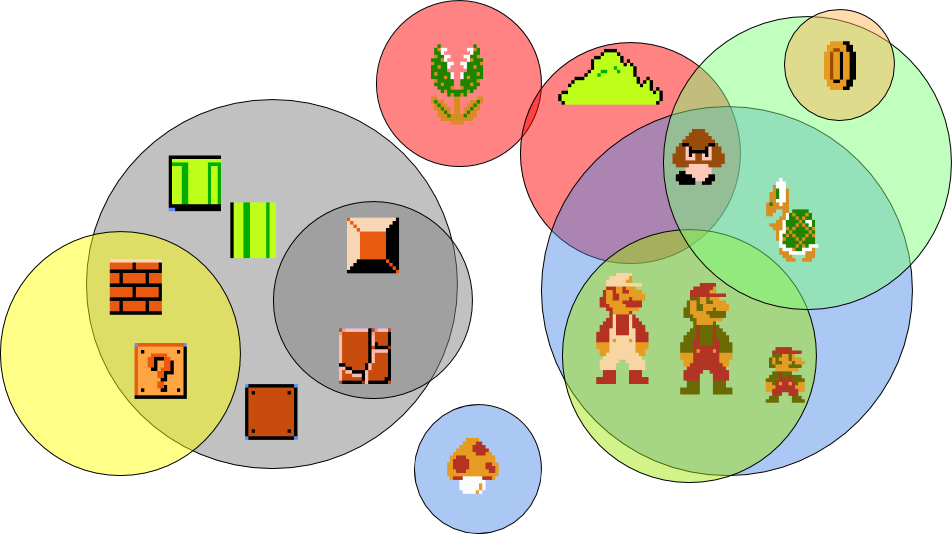
\includegraphics[width=0.97\textwidth]{figures/Clusters.png} 
   
    \caption{Clusters found by \textbf{PMI - Generalized}. \textit{Grey} is solid, \textit{Yellow} produces coins, \textit{Blue} moves, \textit{Green} can be deleted from the top, \textit{Orange} can be deleted from the sides and bottom, \textit{Yellow-Green} can hit ?-Blocks, \textit{Red} harms the character }
  \label{fig:Clusters}
  \end{figure}

We used four different approaches:

\begin{itemize}
 \setlength\itemsep{0.1mm}
\item Pointwise Mutual Information
\item Bayes Nets
\item RESCAL
\item The Infinite Relational Model
\end{itemize}

to find important causal relationships, and cluster them based on their shared properties.  We found that a hybrid approach utilizing Pointwise Mutual Information to first cluster together the most highly causal interactions and then using the Infinite Relational Model to fill in gaps in the coverage had the best overall results with 15 discovered clusters, full coverage of all in-game entities, and an average cluster entropy of 0.07.  The clusters found by Pointwise Mutual Information can be seen in figure \ref{fig:clusters}.  In general the most important mechanical properties have been discovered, with important distinctions being found, e.g. all of the solid tiles (the gray cluster) are found with the fully inert tiles (the smaller gray cluster) being found different than those that have other properties (the breakable block and question mark blocks being able to be changed by collision with Mario) or some oddities (pirannha plants passing through only the pipes, or the solid brown block being the end-state of breakable blocks and question mark blocks).

The above work made some large assumptions about the mechanical properties that might be present, but we might wish to learn these mechanical properties with minimal intervention.  Toward this end, I worked on a system, CHARDA, to learn Hybrid Automata (HA) representations of the game mechanics present for different game entities directly from play traces.   CHARDA recovers the distinct dynamic modes of the HA, learns a model for each mode from a given set of templates, and postulates \textit{causal} guard conditions which trigger transitions between modes. CHARDA first learns which mode is active at each point in the trace via a dynamic programming implementation.  At each sub-interval, we consider all possible mode templates, systems of equations that could possibly explain the observed phenomena, and determine the best possible model for that interval for a given definition of ``best''.  In this work, we considered two criteria, Bayesian Information Criterion and Minimum Description Length, which are similar in form and function, but have different theoretical underpinnings.  Both reward model accuracy and penalize model complexity, with the goal being to find a simple, well founded model.  With each sub-interval considered, we can then construct the optimal assignment over all sub-intervals with a dynamic programming scheme.  From this assignment, we then merge sub-intervals according to the aforementioned criterion, i.e. if merging two intervals into one shared mode improves the balance of accuracy and complexity. 

\begin{figure}[htb!]
\fbox{\parbox{\columnwidth}{
% \begin{center}
% \textbf{Reverse Engineered HA}
% \end{center}
\begin{description}
\item [On Ground] $\dot{y} = 0$ --- Caused by Mario colliding with something solid from above 
\item [Jump(1,2,3)] Three jumps with parameters: \begin{itemize}
\item $\dot{y} := 4, \ddot{y} = -\frac{1}{8} $
\item $\dot{y} := 4, \ddot{y} = -\frac{31}{256} $
\item $\dot{y} := 5, \ddot{y} = -\frac{5}{32} $ 
\end{itemize}  Entered from \textbf{On Ground} when the \textbf{A button} is pressed and $|\dot{x}| < 1$,  $1 \leq |\dot{x}| < 2.5$, or  $2.5 < |\dot{x}| $, respectively
\item [Release(1,2,3)]  $\dot{y} := min(\dot{y}, 3)$ --- Entered from the respective \textbf{Jump} when the \textbf{A} button is released; \(\ddot{y}\) same as respective \textbf{Jump}.
\item [Fall(1,2,3)]  Falling at one of three rates: $\ddot{y} = -\frac{7}{16}$, $-\frac{3}{8}$, or $-\frac{9}{16}$; entered from the respective \textbf{Jump} or \textbf{Release} mode when the apex is reached (\(\dot{y} \leq 0\))
\item [Terminal Velocity(1,2,3)] $\dot{y} = -4$ - Entered from \textbf{Fall} when $\dot{y} \leq -4$.  The initial timestep in the \textbf{Terminal Velocity} state is actually $\dot{y} = -4 + \dot{y}-\lfloor \dot{y} \rfloor$ before being set to $-4$.
\item [Bump(1,2,3)] $\dot{y} := 0$ --- Entered from a \textbf{Jump} or \textbf{Release} when Mario collides with something hard and solid from below; \(\ddot{y}\) same as respective \textbf{Jump} or \textbf{Release}
\item [SoftBump(1,2,3)] $\dot{y} := 1 + \dot{y}-\lfloor \dot{y} \rfloor$ --- Entered from a \textbf{Jump} or \textbf{Release} when Mario collides with something soft and solid from below; \(\ddot{y}\) same as respective \textbf{Jump} or \textbf{Release}
\item [Bounce(1,2,3)] $\dot{y} := 4, \ddot{y} := a$ --- Entered when Mario collides with an enemy from above; \(a\) is given by the respective \textbf{Jump}, \textbf{Release}, \textbf{Fall}, or \textbf{Terminal Velocity} state
\end{description}
}
}
\caption{The true HA for Mario's jump in \textit{Super Mario Bros.}  $:=$ represents the setting of a value on transition into the given mode, while $=$ represents a flow rate while within that mode. %Note that our given constrained learnable class is not expressive enough to learn it precisely.
}
\label{fig:TrueHA}
\end{figure}

\begin{figure}[htb!]
\begin{subfigure}[b]{0.99\textwidth}
\fbox{\parbox{\columnwidth}{
% \begin{center}
% \textbf{MDL Criterion Recovered HA}
% \end{center}
\begin{description}
\item [On Ground] $\dot{y} = 0$ --- Caused by Mario colliding with something solid from above 
\item [Jump] $\dot{y} := [3.97,4.10], \ddot{y} = [-0.140,-0.131] $  --- Entered from \textbf{On Ground} when the \textbf{A button} is pressed
\item [Release] $\dot{y} := [2.10,2.54], \ddot{y} = [-0.430,-0.384] $  --- Entered from \textbf{Jump} when the \textbf{A button} is released
\item [Fall] $\dot{y} := 0, \ddot{y} = [-0.373,-0.359] $  --- Entered from \textbf{Jump} or \textbf{Release }when the apex is reached
\item [Bump]  $\dot{y} := [-1.85,-1.27], \ddot{y} = [-0.324,-0.238]$ --- Entered from \textbf{Jump}  when something solid is collided with from below
\item [Bounce]  $\dot{y} := [3.51,3.82], \ddot{y} = [-0.410,-0.378]$ --- Entered from \textbf{Jump}  when an enemy is collided with from above
\item [Terminal Velocity] $\dot{y} = [-4.15,-4.06]$ --- Entered from \textbf{Jump} or \textbf{Fall} 
% \item [On Ground] $\dot{y} := 0, \ddot{y} := 0$ --- Caused by Mario colliding with something solid from above 
% \item [Jump] $\dot{y} := 4.21 , \ddot{y} := -0.168 $  --- Entered from \textbf{On Ground} when the \textbf{A button} is pressed
% \item [Release] $\dot{y} := 0.617, \ddot{y} := -0.294 $  --- Entered from \textbf{On Ground} when the \textbf{A button}
% \item [Fall]  $\dot{y} := -0.484, \ddot{y} = -0.274$ --- Entered from \textbf{Jump} when the apex is reached or when collision with something solid from above is ended
% \item [Bump]  $\dot{y} := 0, \ddot{y} = -0.363$ --- Entered from \textbf{Jump}  when something solid is collided with from below
% \item [Bounce]  $\dot{y} := 4.00, \ddot{y} = -0.369$ --- Entered from \textbf{Jump}  when an enemy is collided with from above
% \item [Terminal Velocity] $\dot{y} := -4.105$ --- Entered from \textbf{Jump} or \textbf{Fall} 
\end{description}
}
}
\label{fig:MDL_HA}
\caption{HA with MDL as the penalty.}
\end{subfigure}
\begin{subfigure}[b]{0.99\textwidth}
\fbox{\parbox{\columnwidth}{
% \begin{center}
% \textbf{BIC Criterion Recovered HA}
% \end{center}
\begin{description}
\item [On Ground] $\dot{y} = 0$ --- Caused by Mario colliding with something solid from above 
\item [Jump] $\dot{y} := [4.19,4.42], \ddot{y} = [-0.195,-0.181] $  --- Entered from \textbf{On Ground} when the \textbf{A button}  is pressed
\item [Fall]  $\dot{y} := 0, \ddot{y} = [-0.356,-0.338]$ --- Entered from \textbf{Jump} when the apex is reached
\item [Bump]  $\dot{y} := [-2.37,-1.67], \ddot{y} = [-0.289,-0.188]$ --- Entered from \textbf{Jump}  when something solid is collided with from below
\item [Bounce]  $\dot{y} := [3.52,3.88], \ddot{y} = [-0.424,-0.391]$ --- Entered from \textbf{Jump}  when an enemy is collided with from above
\item [Terminal Velocity] $\dot{y} = [-4.16,-4.05]$ --- Entered from \textbf{Jump} when the threshold of $-4$ is reached.
% \item [On Ground] $\dot{y} := 0, \ddot{y} := 0$ --- Caused by Mario colliding with something solid from above 
% \item [Jump] $\dot{y} := 4.37, \ddot{y} := -0.202 $  --- Entered from \textbf{On Ground} when the \textbf{A button}  is pressed
% \item [Fall]  $\dot{y} := -0.484, \ddot{y} = -0.274$ --- Entered from \textbf{Jump} when the apex is reached or when collision with something solid from above is ended
% \item [Bounce]  $\dot{y} := 3.37, \ddot{y} = -0.410$ --- Entered from \textbf{Jump}  when an enemy is collided with from above
% \item [Terminal Velocity] $\dot{y} := -4.05$ --- Entered from \textbf{Jump} or \textbf{Fall} 
\end{description}
}
}
\label{fig:BIC_HA}
\caption{HA with BIC used as the penalty}
\end{subfigure}
%\caption{Learned Mario HAs. Parameters as 95\% CI.}
\caption{Learned Mario HAs. Parameters as 95\% confidence intervals.}
\label{fig:LearnedHA}
\end{figure}



With a segmentation of the trace into these modes, we then learn guard transitions between modes, i.e. under what conditions do we transition from mode $A$ to mode $B$. e.g. In \textit{SMB} Mario transitions from being on the ground to jumping when the A button is pressed. We do this by again using PMI to find which explanatory variables are most likely causing these transitions (e.g. we might observe many different B button presses or collisions with background objects with no change in mode, but the A button press is always found). The HAs learned by CHARDA can be seen in Figure \ref{fig:LearnedHA}, in comparison to the true HAs in \ref{fig:TrueHA}.  The Mario trace used for this work was 3772 frames in length, $~63$ seconds.  The learned HAs are over-approximations of the true HA.  Whereas the true HA has 3 separate jump modes based on the state of $\dot{x}$ at the time of transition, the learned HAs have only one such jump whose parameters are averages of the parameters of the true modes.  Following from learning just one jump, CHARDA learns only a single falling mode.  MDL does learn that releasing the \textbf{A} button while ascending leads to a different set of dynamics, but it considers this a change in gravity as opposed to a reset in velocity.

MDL produces the more faithful model of the true behavior, but is overzealous in its merging of the distinct jump mode chains into a single jump mode chain. As such, it only recovers 7 of the 22 modes; however, abstracting away the differences between the jump chains it learns 7 of 8 modes, only missing the distinction between hard bump and soft bump. 
As an abstraction, this seems similar to what a human analyst might decide.
Any implementation of this algorithm could certainly track which modes were merged and offer to un-merge them in case an analyst believes the elided distinctions are actually important.


\emph{Mappy} is designed to work on games where an \emph{avatar} moves around a large \emph{world} broken up into smaller \emph{rooms}.
This covers significant aspects of a broad class of games including platformers, action-adventure games, and role-playing games.
We based this view of the world on these games' usual composition of four \emph{operational logics}~\cite{wardrip-fruin2005playable,osborn2017refining}: \emph{collision logics}, which describe spaces made up of distinct objects which can touch each other and possibly block each other's movement; \emph{linking logics}, which define larger conceptual spaces including connected rooms and the transit between them; \emph{camera logics}, which account for the fact that the visible part of the world is a window onto a larger contiguous world; and \emph{control logics}, which map e.g.\ button inputs to in-game actions.

Operational logics combine abstract processes (collision detection and restitution, the movement of the player between discrete spaces, the selective drawing of a sub-region of the whole level, or conditional control of the player character) with strategies for communicating these processes to players (tiles and sprites, scrolling or screen-fading to change rooms, continuous smooth scrolling, and ignoring input during cutscene-like segments such as switching rooms).
We find that operational logics provide useful inspiration for knowledge representation and inductive bias; they help structure intuitive observations about how games function in a way that is amenable to automation.
The following sections expand on the leverage we get from operational logics as a knowledge representation.

In its current form, \emph{Mappy} takes as input a playthrough of a game and the game program, then runs an NES emulator on that program and observes the system's state over time.
\emph{Mappy} watches a portion of the screen for changes; this screen rectangle is currently given in advance, but it could be determined automatically in the future.
At each timestep, \emph{Mappy} determines what tiles are visible on the screen, whether the screen is scrolling and if so by how much, and whether the player currently has control over the game (through speculative execution of inputs).
\emph{Mappy} accumulates a map of the current room as the game is played: when \emph{Mappy} sees a new part of a room, it adds those tiles to that room's map.
If a tile in a room changes, \emph{Mappy} also notes that the tile has changed, storing a history of each coordinate's contents over time.
This is important for capturing e.g.\ breakable blocks in \emph{Super Mario Bros.}\ or collapsing bridges.
\emph{Mappy} also watches for cases when the player might be moving between rooms and starts on a new map when the move is complete.
Finally, \emph{Mappy} analyzes the rooms it has seen and suggests cases where two witnessed rooms might actually be the same room so that a human may choose whether to merge them together.

\subsection{NES Pragmatics}

\emph{Mappy} works on NES games because that platform's hardware explicitly defines and supports the rendering of grid-aligned tiled maps (drawn at an offset by hardware scrolling features) and pixel-positioned sprites.
The NES implements this with a separate graphics processor (the \emph{Picture Processing Unit} or PPU) that has its own dedicated memory defining tilemaps, sprite positions (and other data), color palettes, and the \(8 \times 8\) patterns which are eventually rasterized on-screen.
During emulation, \emph{Mappy} can directly read the PPU memory to access all these different types of data; we briefly describe the technical details below (referring the interested reader to~\cite{nesdev}).

Although the PPU has the memory space to track 64 hardware sprites at once, there are two important limitations that games had to contend with: first, each sprite is \(8 \times 8\) pixels whereas game objects are often larger; and second, the PPU cannot draw more than eight hardware sprites on the same \emph{scanline} (screen Y position).
This means that sprites are generally used only on objects that \emph{must} be positioned at arbitrary locations on the screen.

Static geometry, including background and foreground tiles, are not built of sprites but are instead defined in the \emph{nametables}, four rectangular \(32 \times 30\) grids of tile indices; these four nametables are themselves conceptually laid out in a square.
Since the PPU only has enough RAM for two nametables, individual games define ways to mirror the two real nametables onto the four virtual nametables (some even provide extra RAM to populate all four nametables with distinct  tiles).
On each frame, one nametable is selected as a reference point; when a tile to be drawn is outside of this nametable (due to scrolling) the addressing wraps around to the appropriate adjacent nametable.
Note that many game levels are much wider than 64 tiles---the game map as a whole never exists in its player-visible form in memory, but is decompressed on the fly and loaded in slices into the off-screen parts of the nametables as the player moves around the stage.

\emph{Mappy} remembers all the tiles that are drawn on the visible part of the screen, filling out a larger map with the observed tiles and updating that map as the tiles change.
A \emph{Mappy} map at this stage is a dictionary whose keys are a tuple of spatial coordinates (with the origin initially placed at the top-left of the first screen of the level) and the time points at which those coordinates were observed, and whose values are \emph{tile keys}.
A tile key combines the internal index used by the game to reference the tile with the specific palette and other data necessary to render it properly (from the attribute table and other regions of NES memory).
After \emph{Mappy} has determined that the player has left the room (see Sec.~\ref{sec:links}), the map is offset so that the top-left corner of its bounding rectangle is the origin and all coordinates within the map are positive; this is rasterized and output as an image.
We thereby construct the level as it is seen from the perspective of (tile-based) collision logics: the (mostly) static geometry and its (semantically significant) visual appearance over time.

We learn the full history of every tile, rather than committing to its initial or final appearance, for four main reasons.
First, during scrolling, stale tiles are regularly replaced with fresh ones, and in some games this can even happen at the edges of the screen causing visible glitching.
Second, we often fade into or out of rooms (or perform some other animation), and just taking the first- or last- seen tile could lead to unusable maps.
Third, many tiles animate during play (for example, ocean background tiles or glittering treasures).
Finally, the player can interact with many tiles: switches can be flipped, blocks can be broken, walls can be bombed, and so on.
So we must store all the versions of a tile to admit applications like learning tile animations or interactions.
For rasterization and visualization, we generally pick the tile's appearance $25\%$ of the way into its observed lifespan, but this is an arbitrary choice and the generated maps are mainly for human viewing.
A more principled choice might be to take the most common form the tile took during its lifespan.

While in general the nametables are used for terrain and the hardware sprites are used for game characters, there are some exceptions.
Large enemies that do not animate much are often built from background tiles (as in some \emph{Mega Man} bosses and \emph{Dragon Quest} enemies); moving platforms act as terrain but generally must be implemented as sprites.
Objects like movable blocks in \emph{Zelda} or breakable bricks in \emph{Super Mario Bros.}\ are tiles most of the time, but temporarily turn into sprites when interacted with so that they can animate smoothly off of the tile grid.
\emph{Mappy} does not account for these special cases yet.

Because some important level objects are sprites and not tiles, we also hope to learn the initial placements of dynamic game objects in the larger map.
\emph{Mappy} identifies abstract game objects by observing hardware sprites over time using the sprite tracker described in~\cite{summerville2017mechanics}.
This system uses information-theoretic measures to merge adjacent hardware sprites into larger game objects and maintains object identity across time using maximum-weight matchings of bipartite graphs (object identity and positioning in 2D space are natural conclusions to draw from collision logics).
For \emph{Mappy}, we take the first-witnessed position of each object, register those coordinates relative to level scrolling (explained in the next section), and render its constituent sprites into our level maps to capture, for example, that a mushroom pops out of a particular question-mark block.

\subsection{Scrolling}

Although the PPU features hardware scrolling, and (some) of this information persists in the PPU's hardware registers, capturing screen scrolling information is surprisingly subtle.
Games can alter the hardware scrolling registers essentially at any time during rendering, to achieve for example split screens or static menus over scrolling levels (the NES does not support layered rendering, unlike the Super NES).
\emph{Super Mario Bros.}\ and its sequels draw the top part of the screen containing status and score information without scrolling, and then turn scrolling on for subsequent scanlines.
\emph{Super Mario Bros.\ 3} puts status information on the \emph{bottom} of the screen as well, so only a small window of the larger screen scrolls.
These are concrete examples of camera logics, where a portion of the screen is dedicated to a viewport backed by the illusion of a moving camera.
As mentioned above, we register the visible part of the level in a larger tilemap, under the assumption that a rectangular viewport will view a rectangular region of a potentially larger space.

\begin{figure}
  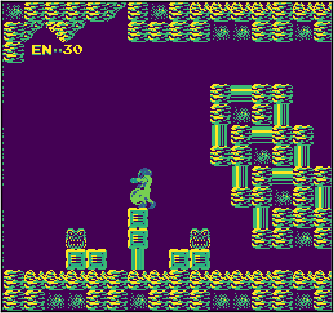
\includegraphics[width=0.44\textwidth]{figures/screen.png}
  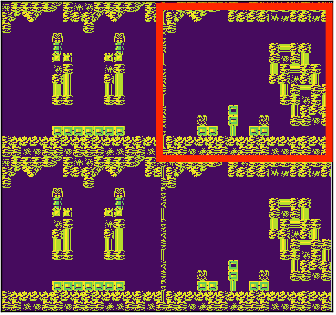
\includegraphics[width=0.44\textwidth]{figures/ntram.png}
  \caption{Visible screen registered with PPU nametables.  Note vertical mirroring and horizontal wrapping.} \label{fig:ntas}
\end{figure}

We could have obtained pixel-precise scrolling information by instrumenting the emulator to trace when hardware scrolling state changes, but we wanted to see how far we could get without such interventions to remain as general as possible.
We deploy two techniques, each with their own strengths and weaknesses: a perceptual algorithm based on registering each frame's visual output with the previous frame's and a hybrid approach which registers only the current frame's visual output (converted to grayscale) with the PPU's four nametables to determine which rectangular sub-region of the larger tilemap is being shown (see Fig.~\ref{fig:ntas}).
The former technique can break down with animated backgrounds (for example, waterfalls), while the latter will fail if the perceived scrolling is done mainly by sprites rather than background tiles, as in certain boss fights in \emph{Mega Man 2}---this would also be an issue if we tracked hardware scrolling with the instrumentation described above.
In either case, once \emph{Mappy} has precise scrolling information it can convert coordinate spaces from the subset of tiles drawn on the screen into the frame of reference of the larger map it is assembling.

\subsection{Linked Rooms} \label{sec:links}


\begin{figure}
\centering
\includegraphics[width=0.48\textwidth]{figures/Metroid.pdf}

\caption{The first four rooms from \emph{Metroid}.  Note that we only observed a small portion of room $1$, which is actually another tall vertical corridor.}
\label{fig:metroid}
\end{figure}

In this work we want to learn not only one large tilemap, but the graph structure by which smaller rooms are linked together (game worlds are not in general planar or even Euclidean).
To do this, we need to determine when the player leaves one contiguous space for another.
We consider two main ways in which linking logics communicate room changes to players:
\begin{itemize}
\item Smoothly scrolling between connected rooms
\item Teleporting between rooms
\end{itemize}
The first type of transition is the most common type in \emph{The Legend of Zelda} and \emph{Metroid} (see Fig.~\ref{fig:metroid}).
In these games, when traversing between most rooms the player loses control for a period of time while the screen rapidly but smoothly scrolls completely into the new room.
After the player regains control, they are in a new room.
To test for this type of transition we must know for each frame whether the screen is scrolling and whether the player has control; we already know about scrolling, so we use the savestate features of the emulator to determine whether the player has control.

The central question of player control is: ``Would the world have been different if the player had done something else?''
Because we know the full input sequence we can look a few moves ahead to see how the world will evolve according to the playthrough; we automatically take a screenshot of that state for reference.
Next, we simulate seven possible futures (one for each button besides ``start'') three frames ahead and compare a screenshot taken in each of those eventualities against the reference state.
If these actions produce different outcomes than the reference, then the player must have control at the initial frame.

In many games, some animations enacted by the player implicitly remove player control for some period of time (e.g.\ the fixed length jumps in \emph{Castlevania}), so we have a configurable parameter for how long control must be taken away before counting as a complete loss of control.
Since most room transitions take at least one or two seconds, and most in-game animations remove control for less time than that, this allows for a clean separation of the two causes for losing control.
Of course, it is conceivable that the player does not have control but is not entering a new room, so we stipulate that the screen must also be scrolling while control is lost (and, indeed, that it must have scrolled by at least half the scroll window width/height).
This accounts for freeze frame animations such as when Mario acquires a mushroom and grows or the fanfare that plays when Samus acquires a new item, which show a loss of control but the screen stays stationary.

The second category of spatial transition above places the player in a new room that has little or no visual relation to the previous room, perhaps from descending a staircase or going down a pipe.
We treat these by looking at the overall appearance of the game screen, and if it changes too drastically within a short timeframe we assume that the player has probably teleported to a new room.
This is complicated by game levels that incorporate drastic sudden changes to the visible portion of the tilemap (such as the ``dark storm'' level in \emph{Ninja Gaiden} or Bright Man's stage in \emph{MegaMan 4}), which yield false positives where \emph{Mappy} thinks that it has gone to a different room.
Given the optional room merging discussed below (and the possibility of stronger heuristics which we leave for future work), we do not believe that this is a fatal flaw.

\subsection{Content Generation}

\label{sec:ContentGeneration}
My work on generating content has been focused on the domains mentioned in the related work, \textit{Super Mario Bros.} and \textit{The Legend of Zelda}.  The generation work has not utilized any of the above mechanical property learning and has so far relied on human semantic compression as in the work of Snodgrass and Onta{\~n}{\'o}n and Dahlskog et al.  

\begin{figure}[ht]
\centering
    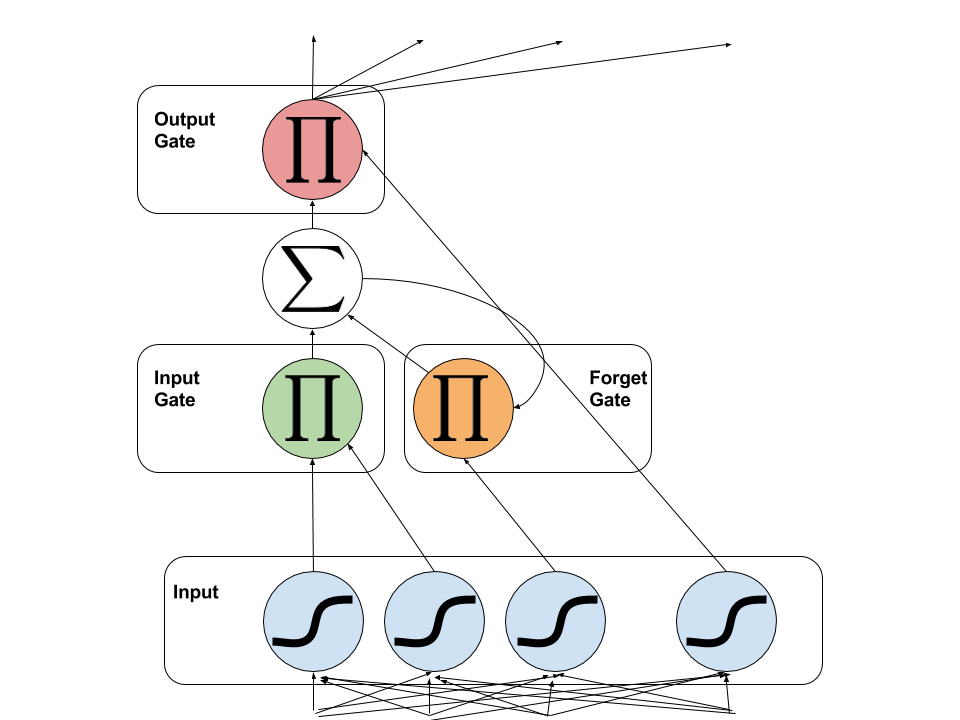
\includegraphics[width=0.5\textwidth]{figures/LSTM_Cell.png}
    \caption{Graphical depiction of an LSTM block. }
    \label{fig:LSTM}
\end{figure}

My work for Mario has focused on using Long Short-Term Memory Recurrent Neural Networks (LSTM RNNs) to generate levels as a sequence of tiles.
LSTMs are a neural network topology first proposed by Hochreiter  and Shmidhuber \cite{LSTM} for the purposes of eliminating the vanishing gradient problem.  LSTMs work to solve that problem by introducing additional nodes that act as a memory mechanism, telling the network when to remember and when to forget.  A standard LSTM architecture can be seen in figure \ref{fig:LSTM}.  At the bottom
are nodes that operate as in a standard neural network, i.e. inputs come in, are multiplied by weights, summed, and that is passed through some sort of non-linear function (most commonly a sigmoid function such as the hyperbolic tangent) as signified by the S-shaped function.  The nodes with $\sum$ simply sum their inputs with no non-linear activation, and the nodes with $\prod$ simply take the product of their inputs.  With that in mind, the left-most node on the bottom can be thought of as the \textit{input} to an LSTM block (although for all purposes it is interchangeable with the node second from the left).  The node second from the left is typically thought of as the \textit{input gate}, since it is multiplied with the input, allowing the input through when it is close to 1, and not allowing the input in when it is close to 0.  Similarly, the right-most node on the bottom acts as a corresponding \textit{output gate}, determining when the value of the LSTM block should be output to higher layers.  The node with the $\sum$ acts as the \textit{memory}, summing linearly and as such not decaying through time.  It feeds back on itself by being multiplied with the second from the right node, which acts as the \textit{forget gate}, telling the memory layer when it should drop whatever it was storing. 

These LSTM blocks can be composed in multiple layers with multiple LSTM blocks per layer, and for this work we used 3 internal layers, each consisting of 512 LSTM blocks.  The input layer to the network consists of a One-Hot encoding where each tile has a unique binary flag which is set to 1 if the tile is selected and all others are 0.  The final LSTM layer goes to a SoftMax layer, which acts as a Categorical probability distribution for the One-Hot encoding.  

LSTM's require a 1-dimensional sequence of inputs, but levels in \textit{Super Mario Bros.} are 2-dimensional.  Converting the 2-dimensional grid to a 1-dimensional sequence requires some form of space-filling curve and we considered 5: 

\begin{figure*}[ht]
\centering
    \begin{subfigure}[t]{0.18\textwidth}
    \centering
    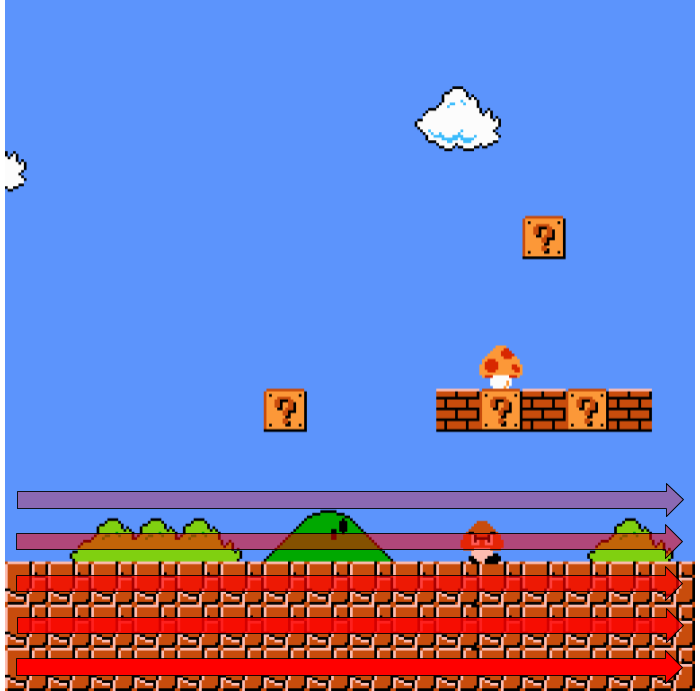
\includegraphics[width=1\textwidth]{figures/Naive.png} 		       \caption{Horizontal}
    \label{fig:naive}
    \end{subfigure}
    \begin{subfigure}[t]{0.18\textwidth}
    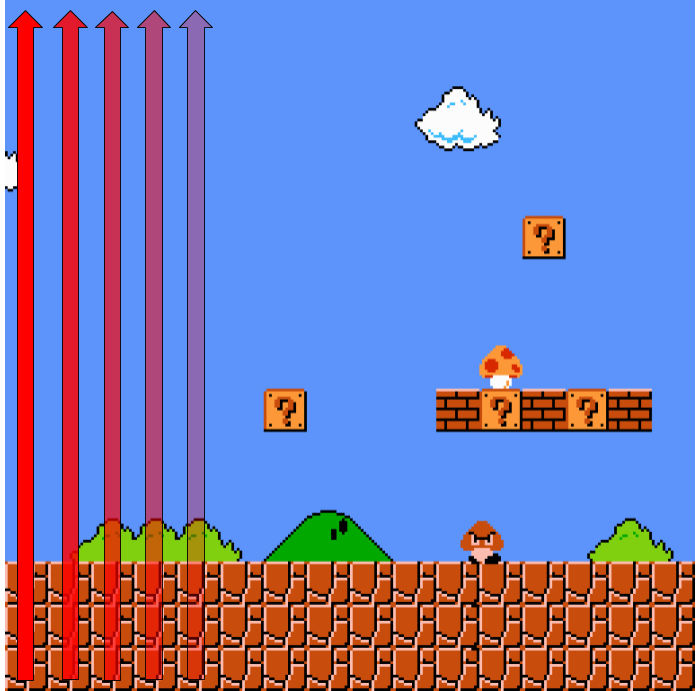
\includegraphics[width=1\textwidth]{figures/BottomToTop.png} 	       \caption{Vertical}
    \label{fig:vertical}
    \end{subfigure}
    \begin{subfigure}[t]{0.18\textwidth}
    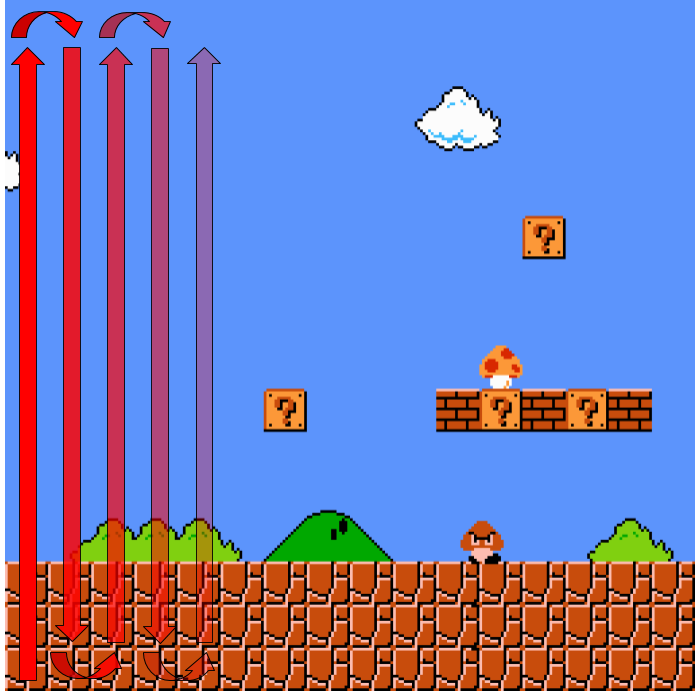
\includegraphics[width=1\textwidth]{figures/Snaking__1_.png} 	       \caption{Snaking}
    \label{fig:snaking}
    \end{subfigure}
    \begin{subfigure}[t]{0.18\textwidth}
    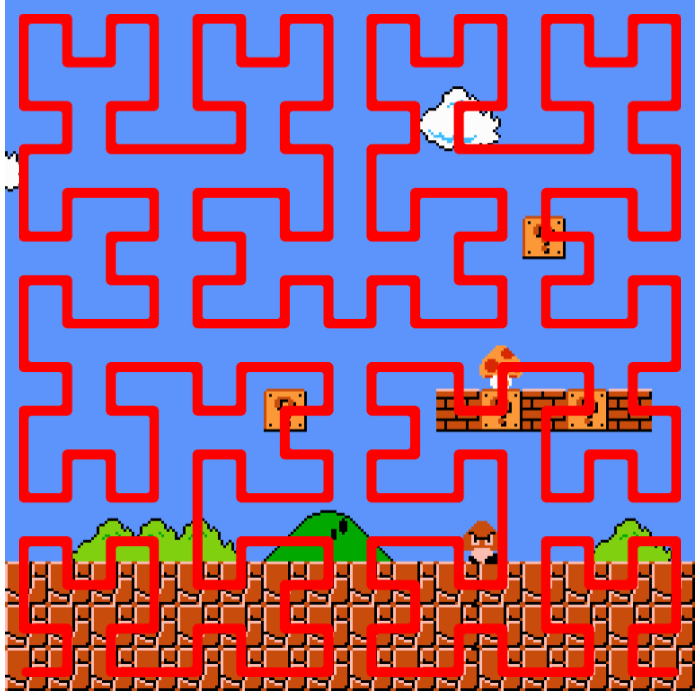
\includegraphics[width=1\textwidth]{figures/Hilbert.png}	       \caption{Hilbert curve}
    \label{fig:hilb}
    \end{subfigure}
    \begin{subfigure}[t]{0.18\textwidth} 
    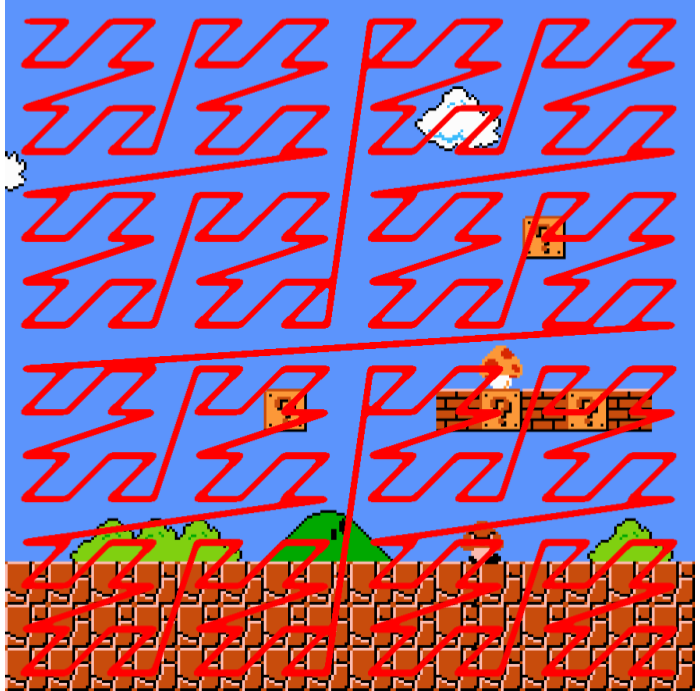
\includegraphics[width=1\textwidth]{figures/Z_Order.png} 	       \caption{Lebesgue curve}
    \label{fig:zorder}
    \end{subfigure}
    \caption{The 1-dimensional orderings considered.}
    \label{fig:orderings}
\end{figure*}


\begin{itemize}
\item \textit{Horizontal} - The ordering progresses from left-to-right and then bottom-to-top.
\item \textit{Vertical} - The ordering goes from bottom-to-top and then left-to-right
\item \textit{Snaking} - The ordering goes from either top-to-bottom or bottom-to-top and when it progresses to the next column (left-to-right) it then reverses (e.g. column 1 is top-to-bottom and then column 2 is bottom-to-top)
\item \textit{Hilbert curve} - The Hilbert curve is a fractal space-filling curve \cite{hilbert1891ueber}.  For this work we used a curve with fractal dimension of 4 (i.e. $16 \times 16$). When a curve ends (if the origin at bottom-left is $<0,0>$ the end point is $<15,0>$) it progresses into another curve (e.g. if the first curve began at the bottom left, the next curve would begin at $<16,0>$)
\item \textit{Lebesgue curve} - The Lebesgue curve is another fractal space-filling curve \cite{morton1966computer}.  Again, we used a curve with a fractal dimension of 4 (i.e. $16 \times 16$)

\end{itemize}

\begin{figure*}[ht]
\centering
    \begin{subfigure}[t]{0.97\textwidth}
    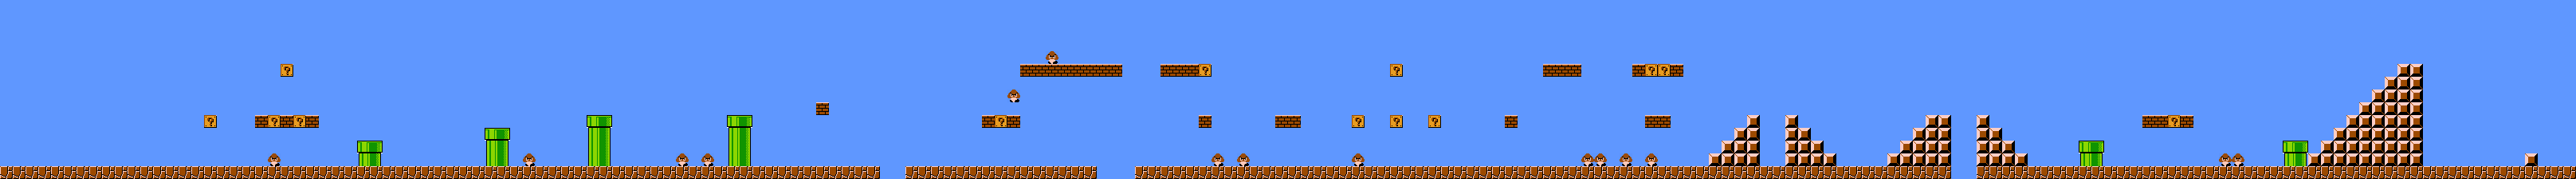
\includegraphics[width=1\textwidth]{figures/1-1.png} 	       \caption{Level 1-1 from \textit{Super Mario Bros.}}
    \end{subfigure}
    
    \begin{subfigure}[t]{0.97\textwidth}
    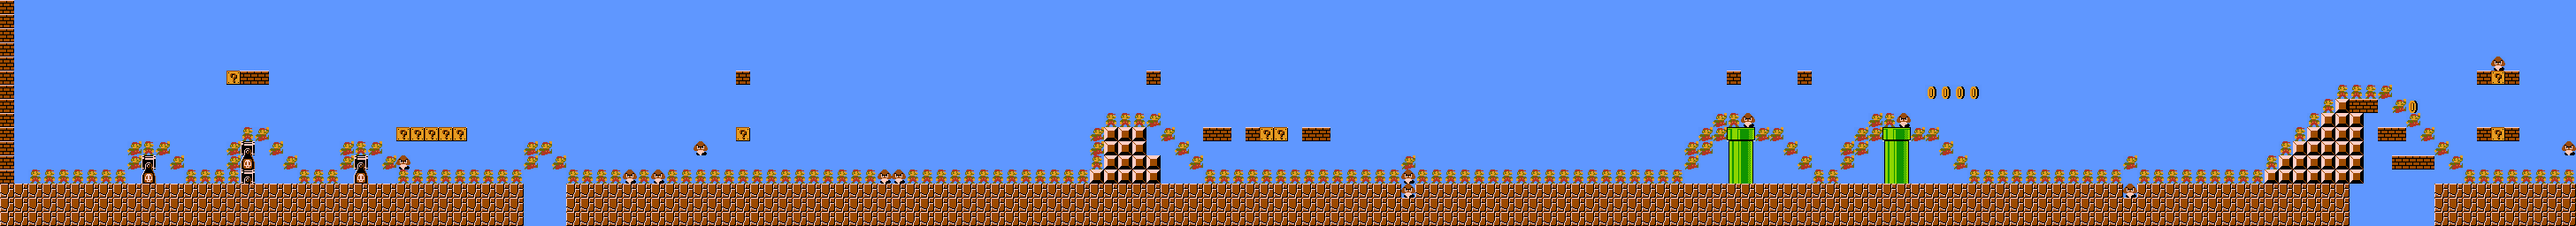
\includegraphics[width=1\textwidth]{figures/SDP1.png} 	       \caption{The generated level from the \textbf{Snaking-Depth-Paths} generator most similar to level 1-1 from \textit{Super Mario Bros.}}
    \end{subfigure}
    \begin{subfigure}[t]{0.97\textwidth}
    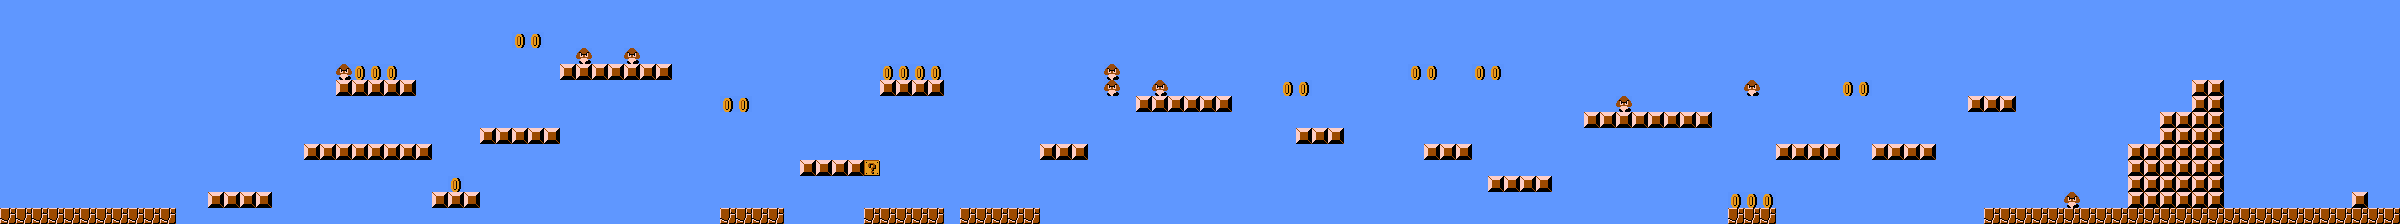
\includegraphics[width=1\textwidth]{figures/1-2.png} 	       \caption{Level 1-3 from \textit{Super Mario Bros.}}
    \end{subfigure}
    \begin{subfigure}[t]{0.97\textwidth}
    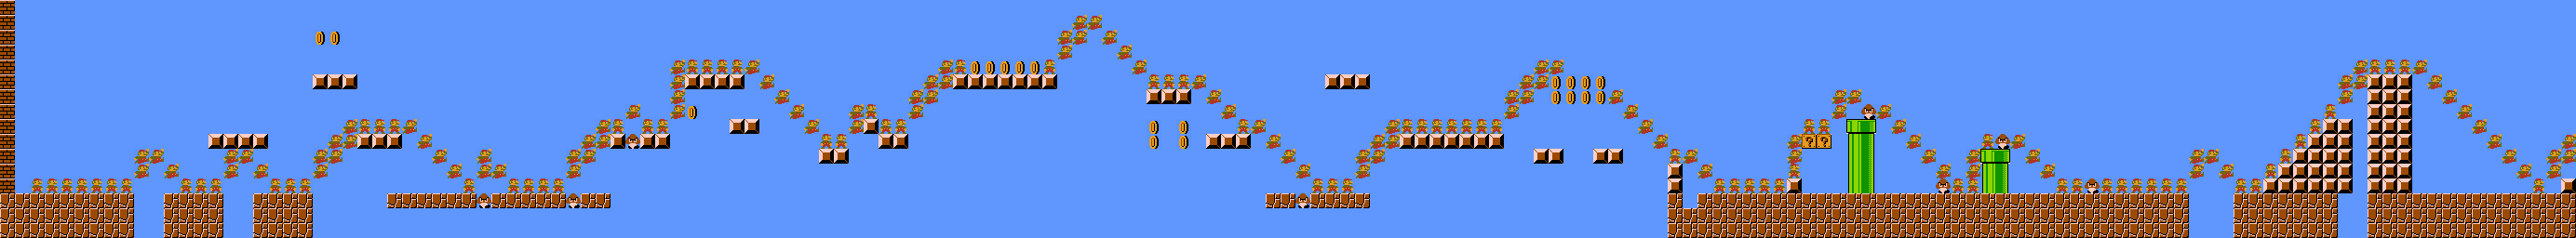
\includegraphics[width=1\textwidth]{figures/SDP_1_3.png} 	       \caption{The generated level from the \textbf{Snaking-Depth-Paths} generator most similar to level 1-3 from \textit{Super Mario Bros.}}
    \end{subfigure}
    \caption{Two levels generated that are most similar to two levels from the original \textit{Super Mario Bros.}  }
    \end{figure*}
which can be seen in figure \ref{fig:orderings}.  We also included meta-information in the inputs beyond just the level geometry.  We also considered ``depth'' information, i.e. how deep into the level the geometry was.  As has been alluded to in some of the human-authored rules, Mario levels often have a progression and flow, starting with low-intensity safe areas, progressing through alternating segments of high and low intensity with a final, end-of-level structure that the player must climb.  By including depth information we were able to help the network learn these long-term structures.  We also included path information from a simulated A$^*$ agent, causing the generator to learn not just how to generate levels, but to also generate exemplar player paths through the level.  Since all training levels had solid, unbroken paths, the generated also had such paths, thereby drastically increasing the percentage of playable levels. Each network was trained on 15 levels from \textit{Super Mario Bros.} and 24 levels from the \textit{Japanese Super Mario Bros. 2}for a total of 39 levels.  Each network then generated 4000 levels.  These levels were then evaluated for whether they were completable.  We also wanted each generator to produce unique levels, and not just memorize from the training set.  We found that the \textbf{Vertical-Depth-Paths} and \textbf{Snaking-Depth-Paths} generators performed the best with 93.30\% and 96.63\% completability rates for the generated level.  In comparison, the highest reported playability results for Snodgrass and Onta{\~n}{\'o}n were 66\% \cite{snodgrassmdmc} and the highest reported for a human-authored system is 94\% for the ORE system of Mawhorter \cite{mawhorterORE}.  Examples of generated levels can be seen in figure \ref{fig:mario_levels}.  The  levels shown were chosen because they were the closest to two original levels across a number of metrics.  Each level has a number of different metrics computed for it.  The metrics are then normalized such that they have a mean of 0 and variance of 1.  The $l^2$ distance is calculated and the closest point is chosen. The metrics considered are: 

\begin{itemize}
\item $C$ - The percentage of the levels that are completable by the simulated agent
\item $e$ - The percentage of the level taken up by empty space
\item $n$ - The negative space of the level, i.e. the percentage of empty space that is actually reachable by the player
\item $d$ - The percentage of the level taken up by ``interesting'' tiles, i.e. tiles that are not simply solid or empty
\item $p$ - The percentage of the level taken up by the optimal path through the level
\item $l$ - The length of the level in number of tiles in width
\item $L$ - The leniency of the level, which is defined as the number of enemies plus the number of gaps minus the number of rewards
\item $R^2$ - The linearity of the level, i.e. how close the level can be fit to a line
\item $j$ - The number of jumps in the level, i.e. the number of times the optimal path jumped
\item $j_i$ - The number of meaningful jumps in the level.  A meaningful jump is a jump that was induced either via the presence of an enemy or the presence of a gap.
\end{itemize}

This method of selecting generated content works not just as a methodology for choosing how to showcase generated content (removing problems of cherry-picking, random selection, and showing that the most similar generated content is not merely regurgitated), but is also a way for a designer to exert control on the generated content.  A designer does not have to encode the rules that they are looking for, they need merely find exemplars.

An extension of this work replaced the simulated A$^*$ agents with paths provided by actual players.  These paths were then able to bias the generation even though the coarse level geometry remained the same across the players.  Due to the incorporation of player paths in the generation process, the generated levels generated paths informed by the player's actions with corresponding impacts on the generated levels.  E.g. a player that interacts with enemies more is more likely to have enemies along their generated path, which in turn means that enemies are more likely to be in the generated level.  We found that the players on the extremes (e.g. those who interact with every interactable object or those who interact with none) had the most biased levels, tailored to those play styles, while ``average'' players in between those extremes had levels most similar to the original \textit{Super Mario Bros.} levels.

 \begin{figure}[htb!]
  \centering
    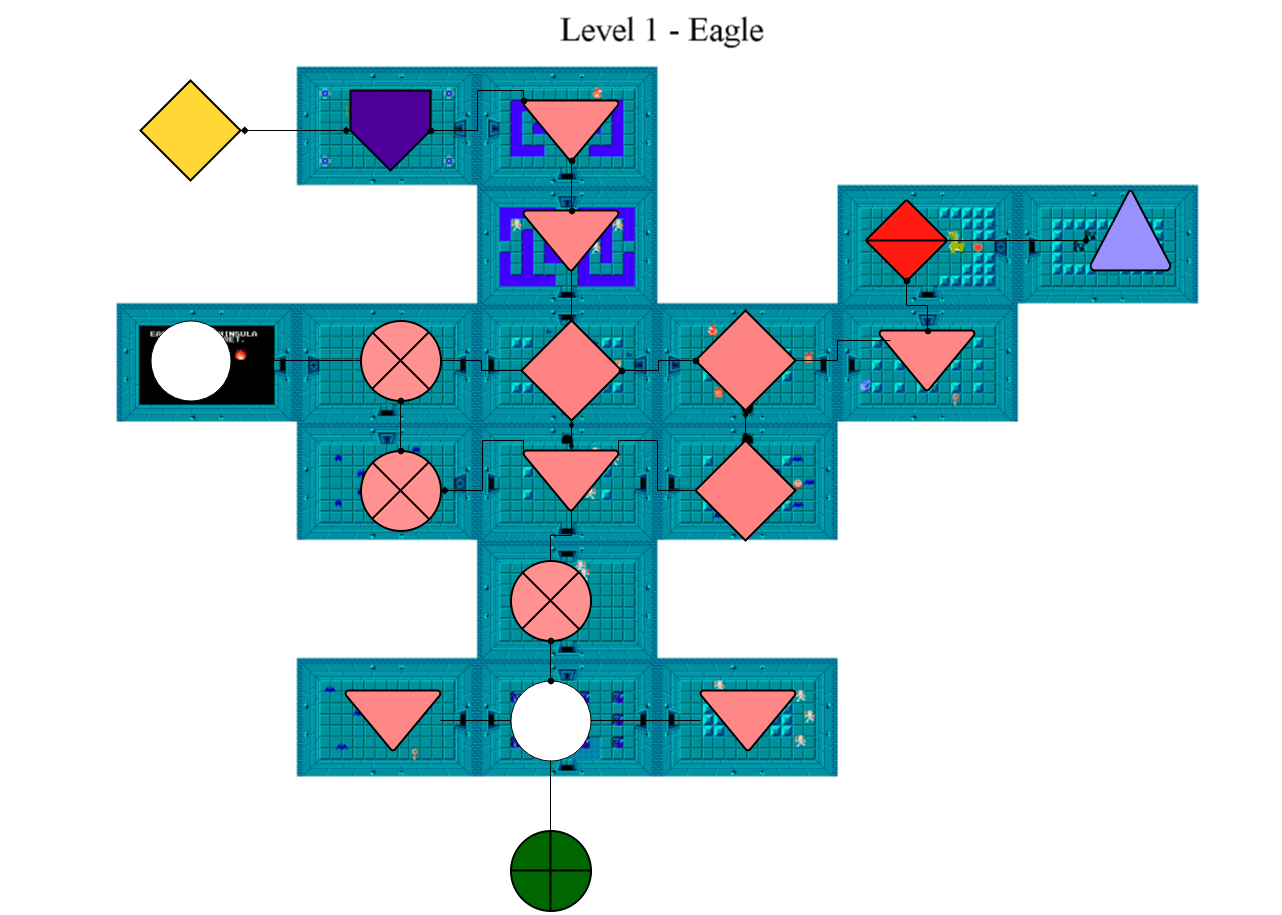
\includegraphics[width=0.95\textwidth]{figures/CopyOfLoz1.png}
  \caption{Annotations for the first level from \textit{The Legend of Zelda}. Green Circle with Plus is the start point. Light Blue Upwards Triangle is the end point. Pink nodes (Diamond, Downwards Triangle, and Circle with X) contain enemies. Downward Triangle nodes contain keys. Diamond nodes contain items. Purple Pentagon nodes contain puzzles. The Red Diamond with horizontal line node contains the boss. The Yellow Diamond off the map shows that it warps to another room}
  \label{fig:Copy_of_LoZ_1}
\end{figure}
As mentioned above, my generation work has not just been limited to \textit{Super Mario Bros.} with work being done for games in \textit{The Legend of Zelda} series.  This work has operated at two different scales, the room-to-room topology of a level and also the in-room tile level construction.  The room-to-room topology is generated using a Bayesian Network (BN) and the in-room tile level utilizes dimensionality reduction via Principal Component Analysis.  To train the BN we annotated existing ARPG levels to be able to extract the relevant features needed. To do this, we used level images from three different ARPGs from the Legend of Zelda series (Fig.~\ref{fig:Copy_of_LoZ_1}). The Legend of Zelda is the progenitor of the genre as well as the genre's most popular series, and, furthermore, is the most prolific series of ARPGs with 17 titles over the course of 28 years. We have used the levels from \textit{The Legend of Zelda}, \textit{The Legend of Zelda: Link to the Past}, and \textit{The Legend of Zelda: Link's Awakening}. We manually annotated 38 levels from the three games and held out 4 levels for our test set. The held out set contained one level from \textit{The Legend of Zelda: Link to the Past} and \textit{The Legend of Zelda: Link's Awakening} each, and two levels from \textit{The Legend of Zelda}. The 34 levels that the model was trained on were composed of 1031 rooms in total, which was the final size of our training set. To annotate these levels, we used images of the levels that show the physical structure of the levels as well as the placement of enemies, items, puzzles, and traps, allowing us to see the full structure of the levels \cite{ZELDASHRINE,ANGELFIRE,ZELDAELEMENTS,IANALBERT}. We then annotate the images to turn them into the graph topology that makes up the \textit{physical space} of the level, where each room is represented as a node in the graph. Nodes (rooms) are annotated by what types of objects it contains: \textit{Start}, \textit{Enemies}, \textit{Puzzles}, \textit{Beneficial Items}, \textit{Keys}, \textit{Big Key}, \textit{Key Item}, \textit{Boss Enemy}, \textit{End}.  A room can contain any number of these elements, although in practice only contain up to 4 of these types of objects.  
 The connections between rooms are annotated with one of the following directed link types:   \textit{Door}, \textit{Bombable Wall}, \textit{Locked Door}, \textit{Soft-Locked Door}, \textit{Big Key Locked Door}, \textit{Key Item Locked Door}, \textit{One Way Door}, \textit{Can See The Other Room}. The \textit{Can See The Other Room} feature is obviously not a standard door but encapsulates an important concept in ARPGs, mainly that the player is often made aware of where they need to go by getting glimpses of another room, but there is no passable edge between their current room and that room.  A sample annotated level can be seen in figure \ref{fig:Copy_of_LoZ_1}.


\begin{figure}[ht]
\centering
  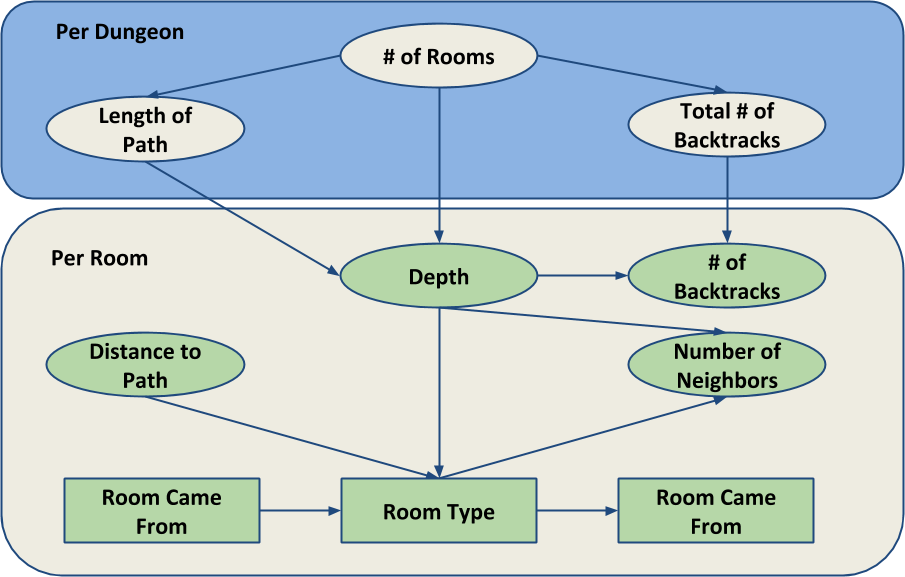
\includegraphics[width=1\linewidth]{figures/The_Learning_of_Zelda.png}
  \caption{}
  \label{fig:BN}
\end{figure}
The trained BN captured a variety of high level features, such as number of rooms in the level and length of optimal path through the level, along with low level features such as room-to-room connections and room types.    At generation time a designer can set whatever they want (or rather \textit{observe} in the Bayesian parlance) and the system will work with that and infer the rest.  e.g. a designer could observe the size of the level, the general make up of rooms, etc..  The system could even be used in a mixed initiative manner with a designer laying out a set of rooms and allowing the system to fill in the rest.  The learned network was composed of the following features:
\begin{itemize}
\item \textit{Number of Rooms in Level}
\item \textit{Number of Doors in Level}
\item \textit{Number of Path Crossings in Level}
\item \textit{Length of Optimal Path}
\item \textit{Distance of Room to Optimal Path}
\item \textit{Path Depth of Room in Level}
\item \textit{Distance From Entrance}
\item \textit{Room Type}
\item \textit{Previous Room Type}
\item \textit{Door Type from Previous Room}
\item \textit{Next Room Type}
\item \textit{Door Type to Next Room}
\end{itemize}


Once the global level parameters have either been observed or inferred, the dungeon is built up from a seed room. The initial entry point to every dungeon is a special \textit{Start} room. \textit{Start} rooms only ever have 1 neighbor, and it is this first neighbor room that is inferred. The room type, the incoming door type, and the number of neighbors are all inferred, given the prior room type (initially the \textit{Start} room), the traversed door type (initially a regular door), its depth in the dungeon (initially one), and all of the inferred or specified global parameters. During this process there is a simultaneous grid embedding process that happens in parallel. The \textit{Start} room is always placed at $(0,-1)$ and its child room is always placed at $(0,0)$. Each new child room is placed at an open neighboring place on the grid, and added to a list of rooms to be inferred. Once all of the specified number of rooms have been placed, a second cleaning process guarantees that the level is playable. d{figure}

For a level to be playable, all of the rooms must be accessible, the number of key locked doors must equal the number of placed keys, all keys must be used to complete the level, all keys must be in front of the doors they lock, and there must be a special item room, a boss room, and an end room. To resolve any of these constraints, we utilize the same machinery that tested the validity of the algorithm, the log-likelihood of a specific event occurring. For example, if there was no end room placed, we simply iterate over all rooms, find the one that has the highest likelihood of being an end room, and change it to an end room. We do this for the boss and special item rooms, in addition to the key locked doors. Once these have been taken care of, we then find the optimal path through the dungeon in order to guarantee that the optimal path through the dungeon uses all of the placed keys. If the level is not completable, then we know that the player is unable to reach a required key. This can be resolved in one of two ways, \textbf{1)} Move a key that has not been reached to a room that has been reached, or \textbf{2)} Move a locked door that has been reached to a door that has not been reached. The choice of how to resolve the violation is chosen at random. On the other hand, if the level is completable, but not all keys are used, then a key-locked door is placed unnecessarily.  To resolve this, an unseen key locked door is moved to a seen unlocked door. No matter what constraint violation is being resolved, it is handled with the same machinery seen above, e.g. if a key needs to be moved, then the existing key room that is least likely to be a key room is removed, and the room it is moved to is the one most likely to be a key room.


\begin{figure*}[ht]
\centering
    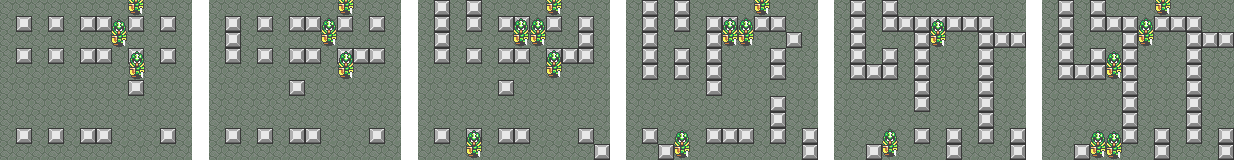
\includegraphics[width=0.97\textwidth]{figures/PCAInterp.png}
    \caption{Interpolation between two human authored rooms.  The rooms on the ends are human authored while the rooms in between represents steps between them of 20\%.}
  \label{fig:PCAinterp}
\end{figure*}

\begin{figure*}[ht]
\centering
    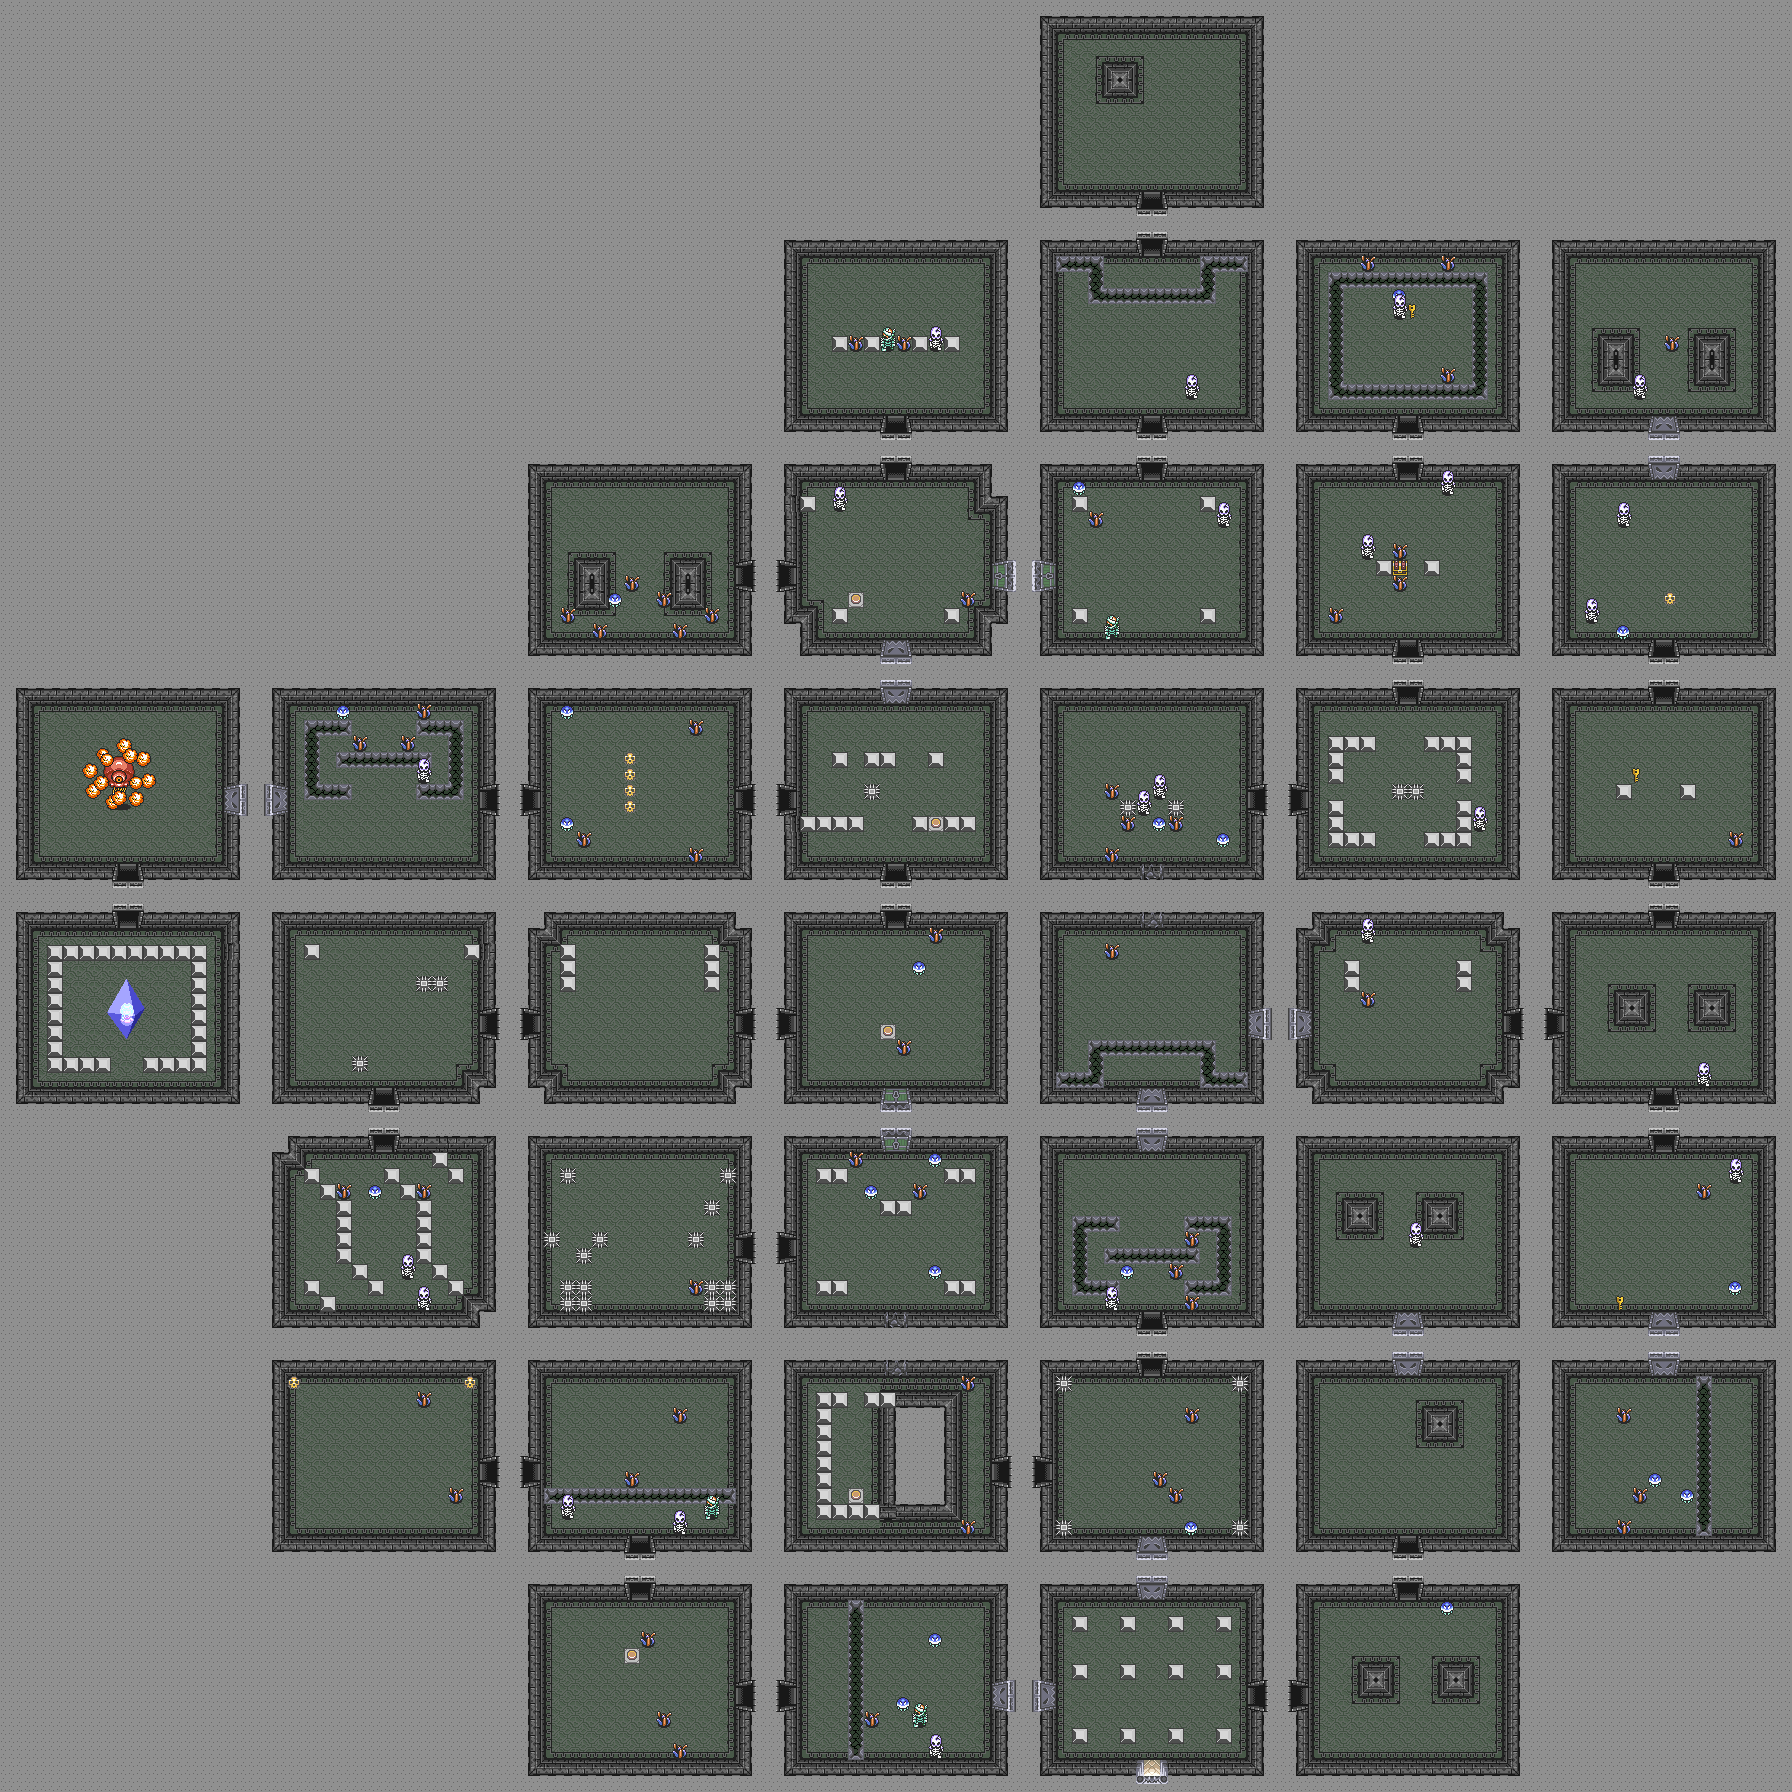
\includegraphics[width=0.97\textwidth]{figures/lttp1.png}
    \caption{A generated level with the most likely high level parameters.}
  \label{fig:dungeon}
\end{figure*}


\begin{figure*}[ht]
\centering
    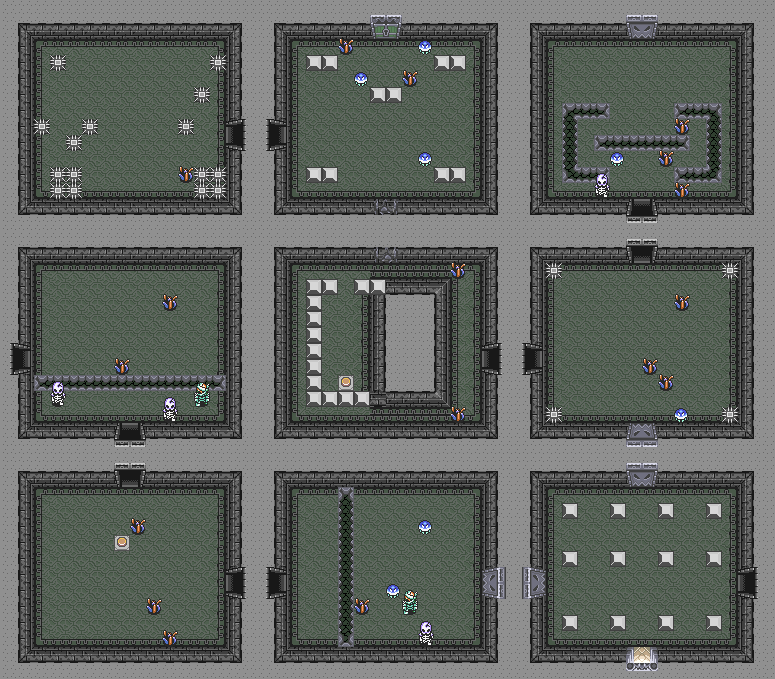
\includegraphics[width=0.97\textwidth]{figures/lttp1_zoom.png}
    \caption{A zoomed in subset, showing the entry point (bottom right corner) and 8 other generated rooms..}
  \label{fig:dungeon}
\end{figure*}
With the level topology constructed we need to generate the rooms at the tile level to have a playable level.  To generate rooms we first performed Principal Component Analaysis (PCA) on a tile level grid representation of the rooms. The dataset for this work was 488 rooms from the three aforementioned games.  However, to increase the size of the sample space we also used all mirrorings (up-down, left-right, both) to quadruple the size of our dataset. Each room can be thought of as a tensor of width by height by tile type, and this tensor is then raveled t make a 1-dimensional vector of size width $\times$ height $\times$ tile type.  All 1952 rooms are converted to this vector format and stacked together to form a 1952 by width $\times$ height $\times$ tile type.  PCA is then applied to this matrix to find a lower dimensionality representation, 20 dimensions in the case covering 95\% of the variance within the data.  To generate a room, existing vectors in this 20 dimensional space are chosen based on the room types (e.g. if a room containing enemies must be generated, 2 vectors corresponding to enemy rooms are chosen) and then randomly interpolated between.  The results of this interpolation can be seen in figure \ref{fig:PCAinterp}. A generated level can be seen in figure \ref{fig:dungeon}, along with a zoomed subset in figure \ref{fig:zoom}.

\subsection{Automatic Game Design}

\begin{figure}[ht]
\centering
    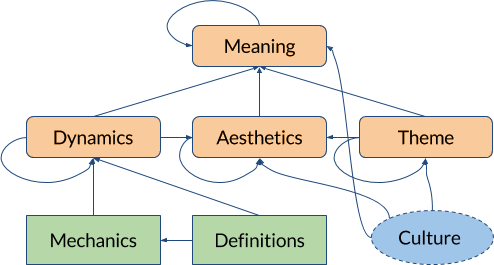
\includegraphics[width=0.97\textwidth]{figures/Proceduralist_Readings_Graph.png}
    \caption{The structure of a proceduralist reading of a game.  Ground facts of the game are green, interpretations are orange, and the cultural knowledge that informs the reading is blue.}
  \label{fig:proc_read}
\end{figure}
  As a part of a larger project designed to procedurally generate narratives paired with matching thematically relevant minigames, I have produced a game generator focused on generating games that afford specific proceduralist readings, a semi-formal approach for interpreting the meaning of a game based on its underlying processes and interactions in conjunction with aesthetic and cultural cues, offer a novel, systematic approach to game understanding.  In proceduralist readings, a game is defined as a set of definitions (entities, resources, etc.) and a set of mechanics.  From these ground facts, the dynamics of play, i.e. what the player will actually do while playing (e.g. if the player has the ability to jump and there exist enemies, the player will jump to avoid them), as well as the aesthetics of play, i.e. how the game actually feels given the dynamics and theming.  These interpretations can be built up to provide high-level readings of the game (e.g. the game of \textit{Kaboom} feels hopeless, since difficulty is always increasing and there is no possibility of winning).  This structure can be seen in figure \ref{fig:proc_read}.
  
In earlier work, the generator portion of the program was turned off, and instead was run only in the proceduralist reading direction, i.e. given a game definition it produces a set of readings for that game.
  

% Brief example
One example carefully studied by Treanor et al. is {\em The Free Culture
Game}, in which ``new ideas'' are represented as floating particles that
must be herded towards producers in the creative commons to keep them
inspired (creating new ideas) and away from the {\em vectorialist}, who
takes ideas out of the creative commons to commodify them for consumers.
The player exerts an indirect force via the mouse cursor on new ideas.
Several proceduralist readings are extrapolated from these mechanics
together with the game's interpretive affordances, such as the colors
selected for producers versus consumers (green versus grey) and the robotic
and malicious audio-visual character of the vectorialist. An annotated screenshot can be seen in figure \ref{fig:fcg_screenshot}.  

\begin{figure}[ht]
\centering
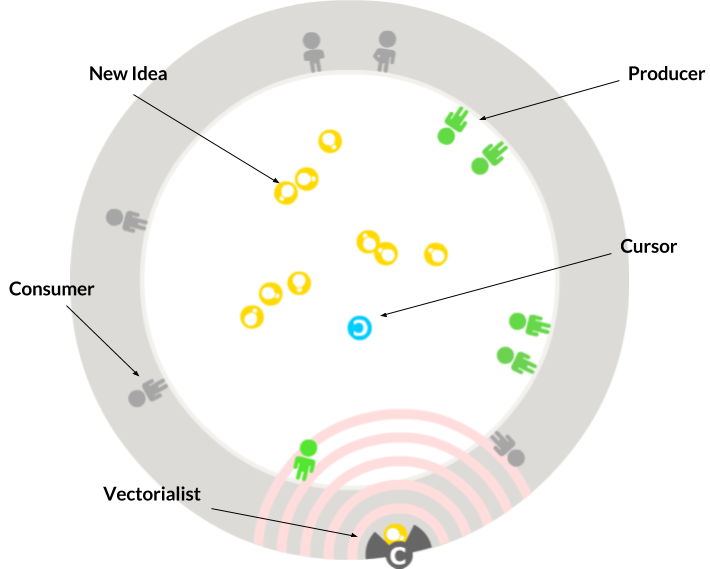
\includegraphics[width=0.95\textwidth]{figures/Free_Culture.png}
\caption{A screenshot of the \textit{Free Culture Game}.}
\label{fig:fcg_screenshot}
\end{figure}

For example, they
read the following meanings from the game:

\begin{enumerate}
\item The player must navigate the cursor between the
  vectorialist and new ideas to prevent commodification.
\item The vectorialist is an evil adversary who does not care
  about the happiness of people.
\end{enumerate}

They derive these meanings from a number of implicit rules, which they call
\emph{dynamics}. We read these as equivalent to~\cite{salen2004rules}'s
\emph{constitutive mechanics}, though we will use the term \emph{dynamics}
here to avoid confusion. For example, the first inference shown on the path to deriving the first reading is:

{\em Because producers need new ideas to collide with them in order not to
turn into consumers, the player's goal is to maintain as many producers as
possible, and the player can exert a force on the new ideas, the player
will push new ideas towards producers. (\textbf{R}eading 1)}

This derivation can be made more explicit by identifying the base
assumptions that can be directly observed about the game (e.g. \textbf{G}oals and \textbf{M}echanics), then building the
argument in a tree structure:


\begin{figure}[ht]
\centering
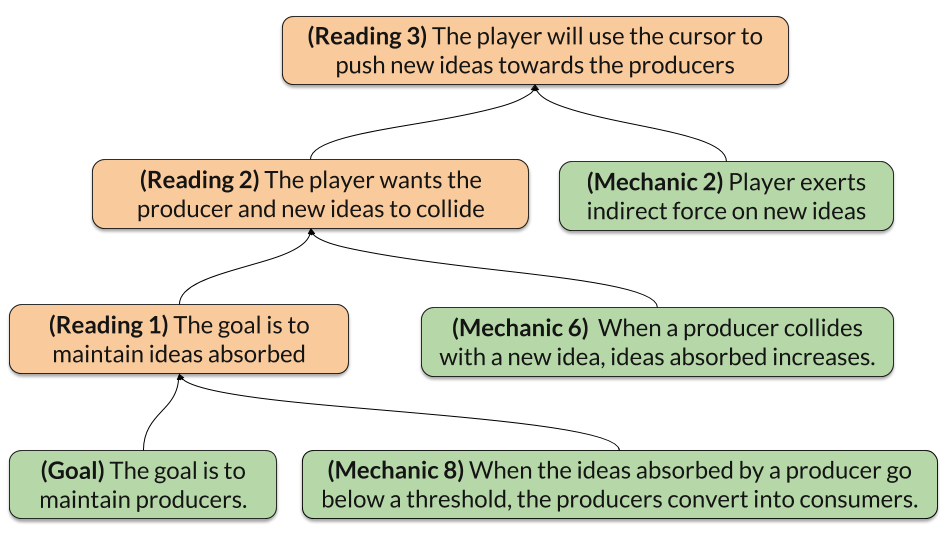
\includegraphics[width=0.95\textwidth]{figures/Copy_of_Proceduralist_Reading.png}
\label{fig:free_culture}
\caption{A color-coded example meaning derivation of an aspect of the aesthetics of the \textit{Free Culture Game}.  \textit{Green} nodes represent concrete pieces of game \textbf{M}echanics and stated \textbf{G}oals that are used as the building blocks for inference chains.  \textit{Orange} nodes represent \textbf{R}eadings, i.e. dynamics such as \textbf{(R1)} are derived from these mechanics and in turn used to derive (also \textit{Orange}) aesthetics such as \textbf{(R2)} and \textbf{(R3)}.}
\end{figure}

Base assumptions:
\begin{itemize}
\item [\textbf{(G)}] The goal is to maintain producers.
\item [\textbf{(M8)}]When the ideas absorbed by a producer go below a threshold, the
producers convert into consumers.
\item [\textbf{(M6)}]When a producer collides with a new idea, the ideas absorbed
increases.
\item [\textbf{(M2)}] The cursor pushes new ideas.
\end{itemize}

Meaning derivation  :

\begin{tabular}{cp{6.5cm}}
 By & \\
 \textbf{(G)}, \textbf{(M8)} & \textbf{(R1)}. The goal is to maintain ideas absorbed.\\
 \textbf{(M6)}, \textbf{(R1)} & \textbf{(R2)}. The player wants the producer and new ideas to collide.\\
 \textbf{(M2)}, \textbf{(R2)} & \textbf{(R3)}. The player will use the cursor to push new ideas toward the
producers.
\end{tabular}


% Identify gap between informal and formal
% Figure~\ref{fig:derivation} depicts the tree structure of this argument
% with the conclusion at the root, premises as subderivations, and definition
% components (mechanics, in this case) at the leaves.  

Characterizing game analysis as a process of constructing these
reasoning structures constitutes an initial step towards a computable
formalism. To operationalize this process, we need to understand the
implicit inference rules that govern {\em why} each proof step is valid.
For example, to state that \textbf{(R1)} follows from \textbf{(G)} and \textbf{(M8)} makes use of the
reasoning that we do as humans about the relationship between goals and
circumstances that defeat those goals.

Some other game reasoning principles that we must codify to fully formalize
the {\em Free Culture Game} meaning derivation include:

\begin{itemize}
\item If the player's goal is $G$ and action $A$ accomplishes $G$, the player will do action $A$.
\item Pushing an entity $E$ with an entity $P$ causes $E$ to move away from $P$.
\item An entity moving away from something might move toward another entity.
\item When $E$ moves toward $X$, $E$ and $X$ might collide.
\end{itemize}

This kind of reasoning is powerfully general in that we can expect to apply
it to many games without having to encode game-specific interpretation knowledge. 
It includes knowledge about player goals and control, causal relationships
between game events, and knowledge about state change phenomena such as
spatial and physical relationships, increase and decrease of resources, the
passage of time, and win and lose conditions. In other words, this kind of
{\em game literacy} must be made explicit in order to perform proceduralist readings.  


We describe game mechanics as a collection of named {\em outcomes} that
have preconditions and results, similar to linear logic-based game
specification in Ceptre~\cite{martens2015ceptre} or the sensors and actors
of Kodu~\cite{stolee2011expressing}. To standardize our game descriptions
in such a way as to describe a broad range of genres, but apply the same
reasoning principles to all specifications, we developed the Cygnus game specification language, which includes the 
aforementioned outcomes as well as notions of
entity, resource, timer, and player controls. Using this formalism, which
we call Cygnus, we can describe the mechanics of {\em The Free Culture
Game} as well as other classic arcade-style games.

A non-exhaustive list of possible preconditions includes:
\begin{itemize}
\item Comparisons of resources: e.g. $R_1 >= 0$
\item Collision detection:  $overlaps(E_1, E_2)$
\item Geometric proximity: $near(E_1, E_2)$
\item Timers elapsing:    $timer\_elapsed(T_1)$
\item Player input:     $button\_press(mouse,held)$
\end{itemize}

A non-exhaustive list of possible results includes:
\begin{itemize}
\item Resource modification:  $R_1 += 2$
\item Entity movement:  e.g. $move(E_1,north)$; $move\_toward(E_1, E_2)$
\item Entity creation/deletion:  e.g. $delete(E_1)$
\item Game mode changes:  $mode\_change(game\_loss)$
\end{itemize}

To carry out automated inquiry about a game, the author creates a
specification of the game's mechanics in Cygnus, then runs the answer set
solver on it in conjunction with the reasoning principles, resulting in a
stable model (collection of logical facts) representing derived knowledge
about the game.  Here we give one example in depth to illustrate the
approach, and we later summarize further efforts for breadth.\footnote{All
code is available at:
\url{https://github.com/LudoNarrative/ClimateChange/tree/master/GameGenerator/Justifications}}

\subsection{The Free Culture Game}

First, we describe our encoding of the \textit{Free Culture Game}'s mechanics in
Cygnus (which we directly embed as ASP predicates). One such mechanic is
{\em The vectorialist pulls in new ideas}, which we describe as an outcome
with a single precondition, {\em the vectorialist is near a new idea}, and
a single effect, {\em the new idea moves toward the vectorialist}. In ASP
predicate notation, we assign this outcome the name \verb|pull_idea| with
the following syntax:

\begin{verbatim}
precondition(
  near(vectorialist, new_idea), 
  pull_idea).
result(pull_idea, 
  move_toward(new_idea, vectorialist)).
\end{verbatim}

The \verb|pull_idea| token is simply an identifier to connect the
precondition to the result, while the \verb|near(-)| and
\verb|move_toward(-,-)| predicates designate specific meanings as preconditions and results in the Cygnus language.



\begin{figure*}

%\begin{verbatim}
%%% (Mechanic 1)
%precondition(slow_timeout, gen_idea).
%result(gen_idea, add(new_idea)).
%
%%% (Mechanic 2)
%precondition(near(cursor, new_idea), 
%  push_idea).
%result(push_idea, 
%  move_away(new_idea, cursor)).
%
%%% (Mechanic 6)
%precondition(overlaps(new_idea, producer),
%  inspire).
%result(inspire, increase(ideasAbsorbed)).
%\end{verbatim}

\begin{verbatim}
%% (Mechanic 1): Producers make new ideas
precondition(slow_timeout, gen_idea).
result(gen_idea, add(new_idea)).

%% (Mechanic 2): The cursor exerts force on ideas.
precondition(near(cursor, new_idea), push_idea(cursor)).
result(push_idea(Entity), move_away(new_idea, Entity))
  :- physicsLogic(Entity, pushing).

%% (Mechanic 3): The vectorialist moves toward groups of new ideas.
precondition(far(vectorialist, new_idea), scan).
result(scan, move_toward(vectorialist, new_idea)).

%% (Mechanic 4): The vectorialist pulls in new ideas.
precondition(near(vectorialist, new_idea), pull_idea(vectorialist)).
result(pull_idea(Entity), move_toward(new_idea, Entity))
  :- physicsLogic(Entity, pulling).

%% (Mechanic 5): Collision between new ideas and vectorialist
%%                kills new idea & increases old ideas.
precondition(collide(new_idea, vectorialist), commodify).
result(commodify, delete(new_idea)).
result(commodify, increase(old_ideas, med)).

%% (Mechanic 6): Collision between new idea & producer increases
%                ideasAbsorbed.
precondition(collide(new_idea, producer), learn).
result(learn, increase(ideasAbsorbed, mid)).
result(learn, set_color(producer,green)).

%% (Mechanic 7): ideasAbsorbed decreases with time.
precondition(tick, forget).
result(tick, decrease(ideasAbsorbed, low)).
result(tick, set_color(producer,gray)).

%% (Mechanic 8): If ideasAbsorbed goes to 0, producer turns into consumer.
precondition(le(ideasAbsorbed, 0), convert_producer).
result(convert_producer, delete(producer)).
result(convert_producer, add(consumer)).

%% (Mechanic 9) (only referred to later than 1st example):
%%  If ideasConsumed goes to 0, consumer turns into producer.
precondition(le(ideasConsumed, 0), convert_consumer).
result(convert_consumer, delete(consumer)).
result(convert_consumer, add(producer)).

%% (Mechanic 10) (only referred to later than 1st example):
%% Vectorialist provides consumers with old_ideas
precondition(gt(old_ideas, 0), feed_consumer).
precondition(near(vectorialist, consumer), feed_consumer).
result(feed_consumer, decrease(old_ideas, low)).
result(feed_consumer, increase(ideasConsumed, low)).
precondition(tick, forget_old).
result(forget_old, decrease(ideasConsumed, low)).
\end{verbatim}

\caption{Formal specification of the mechanics of the \textit{Free Culture Game} in Cygnus.}
\label{fig:fcgformal}
\end{figure*}

\begin{figure}
\begin{verbatim}
%% Initializations
initialize(set_to(ideasAbsorbed,10)).
initialize(set_sprite(producer, person)).
initialize(set_color(producer,green)).
initialize(set_sprite(consumer, person)).
initialize(set_color(consumer,gray)).
initialize(set_sprite(vectorialist, 
  evil_robot)).
initialize(set_color(vectorialist,black)).

%% (Goal) The goal is to prevent producers 
%% turning into consumers.
goal(prevent(convert_producer)).
\end{verbatim}
\caption{Auxilliary clauses for the \textit{Free Culture Game}.}
\label{fig:fcgaux}
\end{figure}

We encode the rest of the game in a similar fashion; we will describe them
in-line with informal descriptions of preconditions and results. The
interested reader may refer to Figure~\ref{fig:fcgformal} for the encoding of
these rules as ASP predicates.
For example, the following three mechanics establish the relationships
between producers, new ideas, and the player:

\begin{itemize}

\item (Mechanic 1): ``Producers make new ideas.'' Precondition: a slow
repeating timer goes off. Result: a new idea is added to the game in a
random location.

\item (Mechanic 2): ``The cursor exerts force on ideas.'' Precondition: the
cursor is near a new idea. Result: the new idea moves away from the cursor.

\item (Mechanic 6): ``Collision between a new idea and a producer increases
ideas absorbed for that producer.'' Precondition: a new idea and a producer
overlap. Result: the producer's ideas absorbed resource increases, which is
reflected by the producer shifting in color from grey to green.

\end{itemize}

In addition to specifying mechanics, we may also supply facts about the
initial state of the game and the game's goal, such as {\em The player's
goal is to prevent producers from converting into consumers.}
See Figure~\ref{fig:fcgaux} for these auxilliary clauses.
\begin{figure*}[h]
\centering
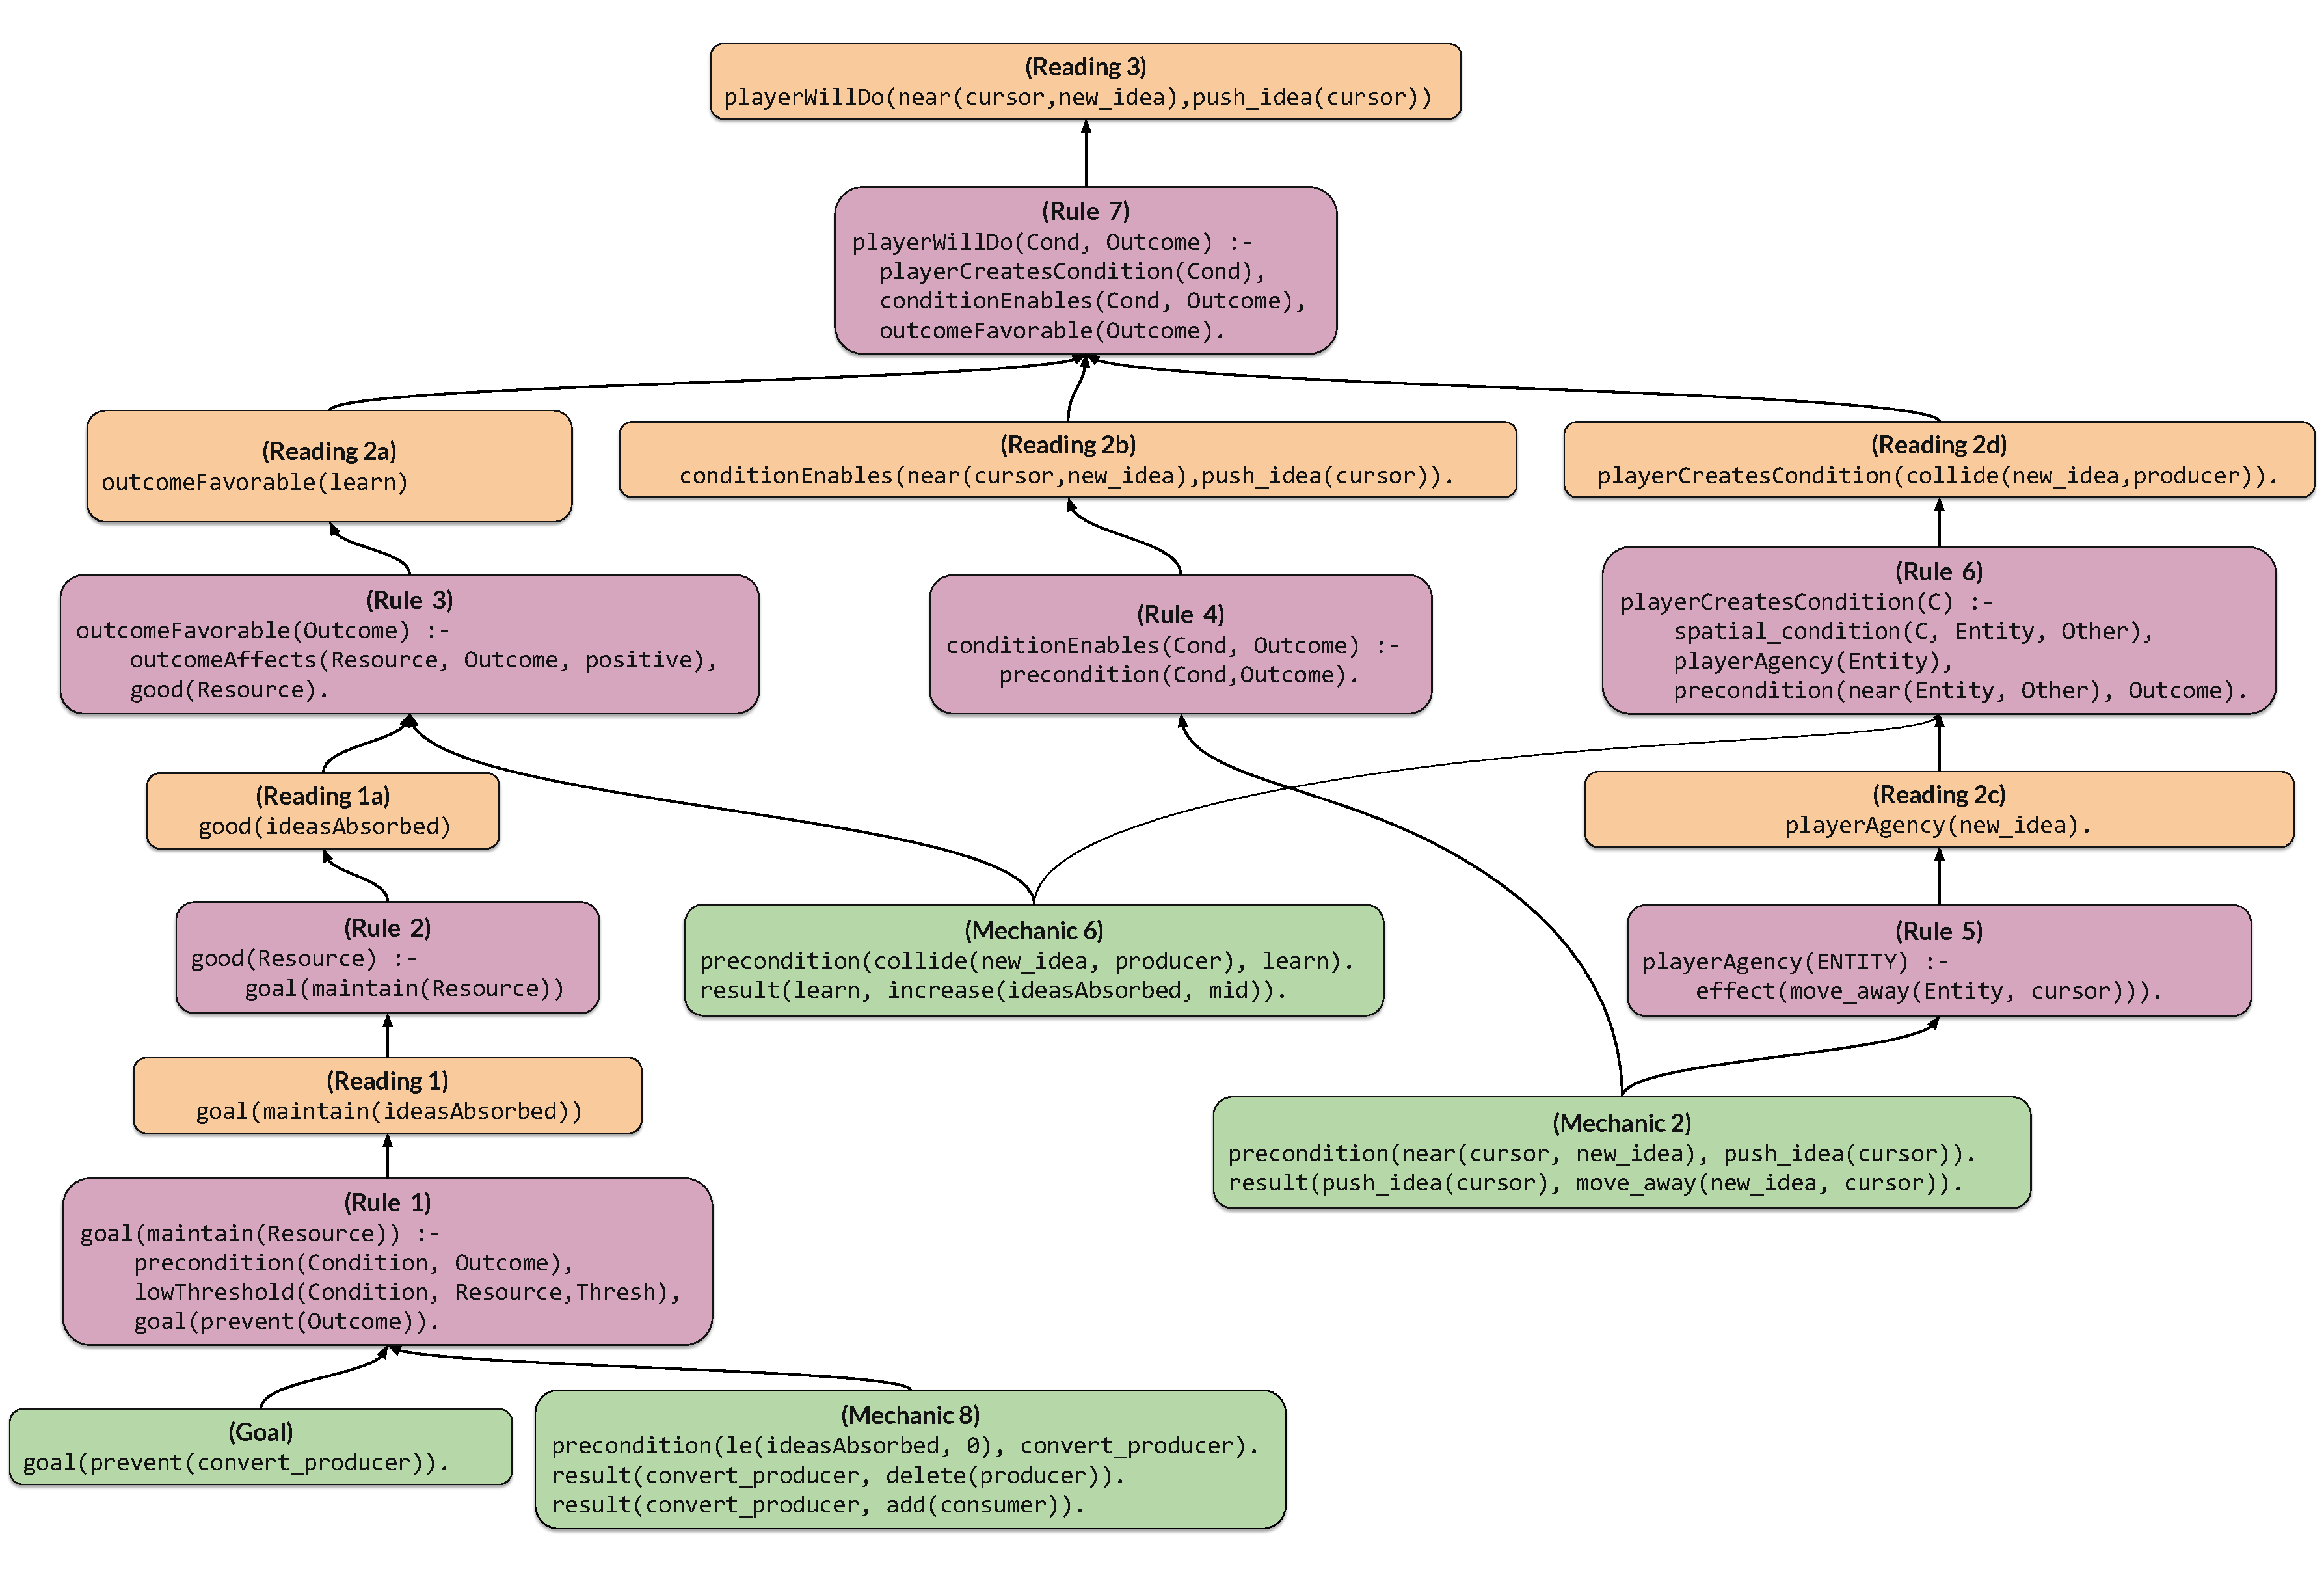
\includegraphics[width=1\textwidth]{figures/-Proceduralist_Reading_-_CODE.pdf}%{-Proceduralist_Reading_-_CODE.png}
\caption{A full reasoning chain, analagous to the prose interpretation found in figure \ref{fig:free_culture}.  The rules invoked in the reasoning are chain are found in purple.  As can be seen, numerous rules and sub-facts might need to be invoked to build up to larger pieces of knowledge, such as the chain building up to \textbf{Reading 2a} ``The outcome labeled `learn' is favorable'' which builds off of 3 separate game definitions and invokes \textbf{Rules 1}, \textbf{2}, and \textbf{3}.}
\label{fig:proc_reading_code}
\end{figure*}

% \begin{figure}[h]
% \begin{verbatim}
% goal(maintain(ideasAbsorbed))
% outcomeAffects(ideasAbsorbed,forget,negative)
% outcomeAffects(ideasAbsorbed,learn,positive)
% outcomeFavorable(learn)

% playerAgency(cursor)
% entityInfluences(cursor,push_idea(cursor))
% enables(push_idea(cursor),learn)

% playerWillDo(near(cursor,new_idea),
%              push_idea(cursor))

% destroys(vectorialist,new_idea)
% requiredBy(new_idea,push_idea(cursor))
% antagonist(vectorialist)

% outcomeBetterThan(producer,initial,forget)
% outcomeBetterThan(producer,learn,forget)
% \end{verbatim}
% \caption{A subset of facts derived for the Free Culture Game.}
% \label{fig:answerset}
% \end{figure}

We pass our reasoning principles and game specification to an answer set
solver, specifically Clingo \cite{clingo}. The solver determines a set of
facts (an answer set) that is consistent and complete with respect to all
axioms and rules provided. This will include all facts derivable from the reasoning principles about the specified game mechanics.

The answer set generated when given the game specification for the Free
Culture Game includes the following facts:

% XXX reformat
The goal is to maintain \verb|ideasAbsorbed|. The outcome  \verb|forget|
affects \verb|ideasAbsorbed| negatively, and the outcome \verb|learn|
affects it positively, meaning that \verb|learn| is a favorable outcome.
The player has agency over the cursor and uses the cursor to influence the
outcome \verb|push_idea(cursor)| which in turn enables the outcome
\verb|learn| by pushing ideas towards the producers.  As such \verb|learn|
is a favorable outcome that the player has indirect control over via
pushing ideas with the cursor, so the player will place the cursor  near
\verb|new_idea|s to try to enact the \verb|learn| outcome.  A graphical representation of these inferred properties along with the rules that were required to derive these can be seen in figure \ref{fig:proc_reading_code}.

However, this is for simply reading a game.  To generate a game, we instead fix a reading, e.g. the game must represent sharing, and generate a game that affords that reading.  The same rules that produce the above reasoning chains are used, but a host of additional rules are required for generation.  The pipeline for game generation is:

\begin{enumerate}
\item Generate partial Cygnus game definitions using ASP
\item Determine scalar values found in rules (e.g. boolean comparisons or modification of other scalar values) using EC
\item Compile complete Cygnus game definitions to Phaser (a javascript game library)
\end{enumerate}

\subsubsection{ASP Game Generation}

As mentioned above, a game is defined by the base objects (entities, resources, timers, etc.) and the rules that govern the game.  All aspects of a game are generated by our system, with minimal guidance from a user only limiting the state-space complexity (e.g. limiting the system to producing games that have at most 3 entities) and the desired readings.  A construct available in ASP is the choice rule, which allows the system to non-deterministically choose whether a predicate exists in the answer set or not.  While the readings are devoid of choice rules, choice rules make up the bulk of the generative aspect, i.e. choosing how entities behave and what rules exist.  The generator can choose:

\begin{itemize}
\item How many entities exist
\item How many resources exist
\item How many timers exist
\item How entities are visually represented
\end{itemize}

to describe the base definitions of the game, but it is in the rules and interactions that govern these entities and resources that the game is found.

The generator chooses how many outcomes can exist and then builds up their preconditions and actions.  The preconditions available are:
\begin{itemize}
\item Whether collision between entity $A$ and entity $B$ is or is not occuring (note, $A$ and $B$ refer to classes of entities and in fact $A=B$ is possible)
\item Whether a resource is above or below a threshold
\item Did the player click on entity $A$ in the last frame
\item Did the player press a button in the last frame
\item Was a button held down in the last frame
\item Did a timer elapse in the last frame
\end{itemize}

In addition to these, there is a default precondition referred to as \textit{tick} which automatically fires every frame of the game.

The possible actions of an outcome are:

\begin{itemize}
\item Modify resource $A$ by either adding or subtracting value $B$ from it
\item Add $C$ entity $A$'s at location $L$
\item Delete entity $A$
\item Move entity $A$ towards or away from entity $B$ at speed $C$
\item Move entity $A$ towards or away from the cursor at speed $C$
\item Move entity $A$ in direction $D$ (where the set of possible directions are either global North, South, East, and West or relative Forward, Backward, Left, Rotate)
\item Rotate entity $A$ by $D$ degrees clockwise or counterclockwise
\item Set entity $A$'s rotation to a random integer between $min$ and $max$
\item Apply collision restitution between entity $A$ and $B$ such that they no longer interpenetrate
\end{itemize}

These preconditions and actions allow for a very expressive set of mechanics to be realized, with mechanics from games such as \textit{Super Mario Bros}, \textit{Asteroids}, \textit{Frogger}, etc. being either nearly or completely realizable.  However, the possibility space afforded by these outcomes is extremely large, and contains many games that are completely unplayable (literally in the case of generated games not allowing for player controls).  

To rein in the space of generated games, a large number of constraints have been authored that attempt to automatically preclude undesirable games.  These are independent of the desired reading of the game and apply to all generated games.  Most are designed to prune out potential rules that while feasible in a game, would not be understandable by a human, such as:


\begin{verbatim} 
:- result(O,move(E,_)), result(O,delete(E)).
\end{verbatim}
   
Which can be read as "It should not be the case that an entity is both deleted and moved by the result of an outcome."  In this case, while technically feasible in the game, the entity would be deleted and therefore it would be impossible to see its motion.  This mechanic is eliminated for 2 reasons:

\begin{enumerate}
\item It would be interpreted solely as deletion of the entity, so it just adds needless size to the solution space for the constraint solver to search through
\item Since the mechanic would result in the deletion, and not movement, of the entity, further rules would have to have added complexity to handle this combination since na\"ively looking for \texttt{result(O,move(E))} expecting movement could be a mistake.
\end{enumerate}

Others are designed to remove games that will deadlock, i.e. gating the increasing of a resource value by a $\ge$ comparison on that resource.  

Once the base rules of a game have been generated, it is balanced via an EC algorithm. The base structure of the game leaves out constant scalar values, e.g.  The following precondition would be generated with ASP


\begin{verbatim} 
precondition(compare(ge,resource(r(1))),outcome(o(1)).
\end{verbatim}
   
Which means that we are checking to see if \texttt{r(1)} $\ge$ some value, but that value is unspecified.

While it would be possible to choose parameters as part of the ASP generation process, we wanted an approach that would allow for multiple non-deterministic play outs of a game in a reasonable time frame, which through trial we found to be infeasible via ASP. 

We consider a population of 50 game tunings.  Each is run through 50 coarse simulations for 20 timesteps.  At each timestep, preconditions for rules are checked.  If a rule is deterministic and must fire, it does.  Conversely, if a precondition for a rule is violated it does not fire.  For non-deterministic rules for which all preconditions are satisfied, it will be randomly chosen according to a simple player model.  Since creating a General Game Player (GGP) is an open field of research \cite{GGPSTUFF}, the simulated play is very coarse and the player model even moreso.  However, our simulated player can leverage the sophistication of the game generation to bias rollouts intelligently.  As part of the generation process, we perform a large amount of reasoning about the outcomes, including whether an outcome is desirable or not.  Instead utilizing  something like MCTS to choose rules based on further simulated play, we can choose outcome that a player will want to enable more heavily than those that come with more tradeoffs and even more heavily than those that will harm the player.  

The fitness of a given tuning is defined as:

$F = O*(S_O-C_O) + E\sum_{O_{mc}}D-\mathrm{earliest}(O_{mc})+\mathrm{latest}(O_{mc}) - S\sum_{O_r} D-\mathrm{seen}(O_r)  $

Where $O$ is a parameter (1000 for this work) to penalize the difference between $S_O$ the number of seen outcomes and $C_O$ the total number of outcomes found. $E$ is a parameter (10) to penalize a mode changing outcome (win or loss) early ($D-\mathrm{earliest}(O_{mc})$) where $D$ is the maximum depth of the simulation and $\mathrm{earliest}(O_{mc})$ is the earliest that outcome $O_{mc}$ is seen, while also rewarding mode changing outcome near the end of the rollout $\mathrm{latest}(O_{mc})$. The final parameter $S$ (1) applies a penalty if a non mode changing outcome $O_r$ for each timestep it is never seen at (i.e. the difference between the rollout depth $D$ and the number of timesteps that outcome is observed at $seen(O_r)$).  This fitness very heavily penalizes games in which an outcome is never seen (presumably due to some mistuning of the parameters), then is hopefully tuned such that it will be won or lost close to the end, and finally wants to be tuned such that any given (non mode changing) outcome can always fire, i.e. no deadlocks.  The EC is run for 50 generations, at the end of which we have a fully specified Cygnus game.   We then compile the Cygnus code to work within the Phaser \cite{phaser} framework, a javascript game engine for 2D games.  

\section{Proposed Work}

\textit{Hylia} is composed of three subsystems: \textit{Nayru}, \textit{Farore}, and \textit{Din} which I will now describe.

\subsection{Nayru --- Game Knowledge Extraction}
\begin{quotation}
\textit{Nayru poured her wisdom onto the earth to give the spirit of law to the world.} \\ \indent  \indent --- Ocarina of Time
\end{quotation}

\textit{Nayru}, named after the goddess of wisdom, is the subsystem that observes games and learns the behaviors and level information contained within.  This section will first provide an overview of the architecture of \textit{Nayru} and then detail the work that still remains to be done.



\begin{figure*}[h]
\centering
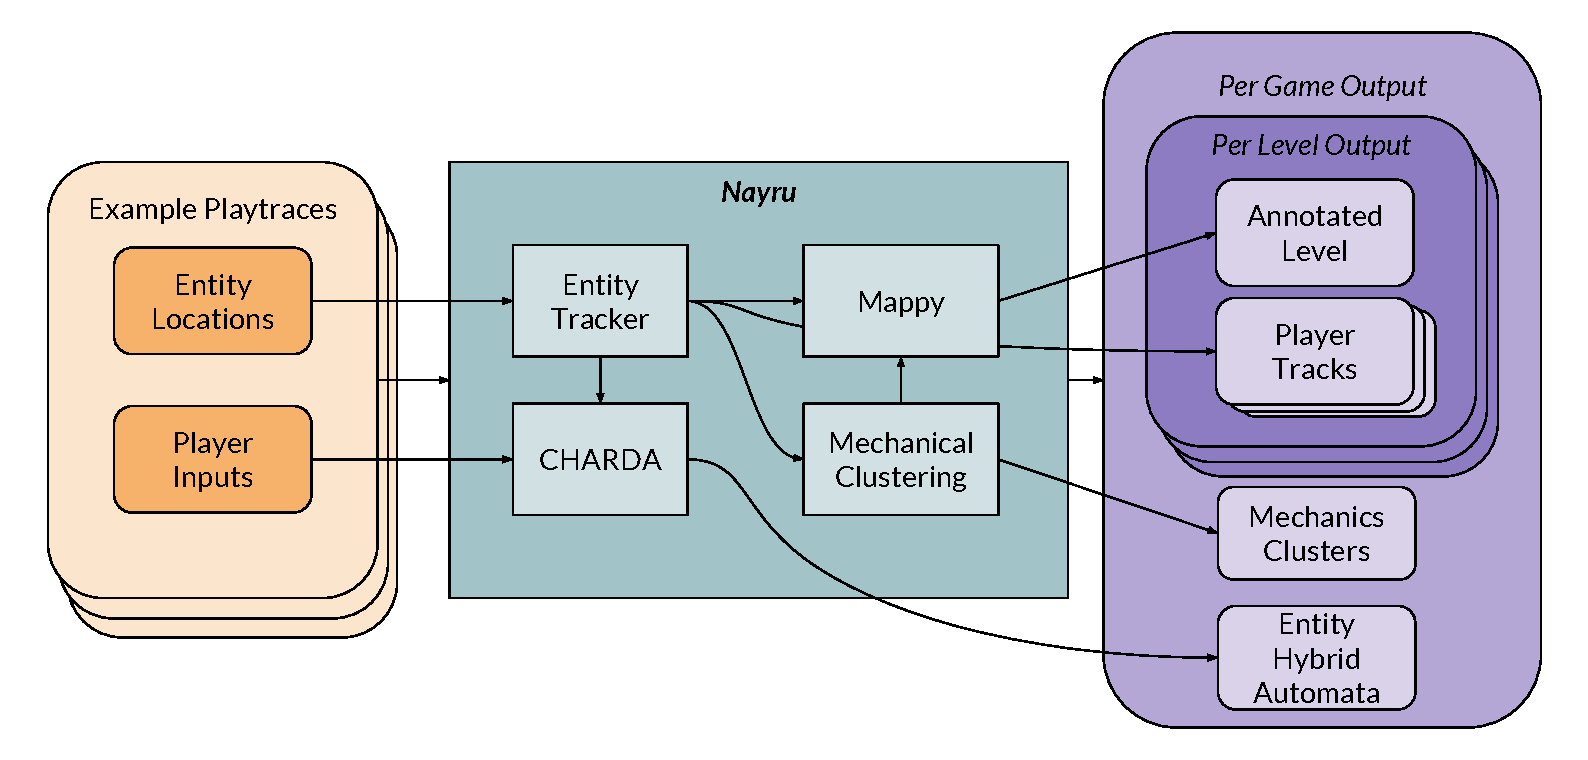
\includegraphics[width=1\textwidth]{figures/Nayru_Architecture.pdf}
\caption{The proposed architecture of \textit{Nayru}.  \textit{Nayru} takes in play traces in the form of entity locations and player input pairs on a per-frame basis.  These pairs are processed by an entity tracker, which is used as input for \textit{CHARDA} and \textit{MAPPY}, which respectively produce Hybrid Automata behaviors and levels.  The levels  }
\label{fig:nayru_architecture}
\end{figure*}

\subsubsection{Nayru Architecture}
The goal of \textit{Nayru} is to be as general as possible with regards to its input, hence it is agnostic of the platform taking in pairs of entity locations and player inputs.  In practice, my thesis work will focus on games from the NES given the framework that I have previously developed for \textit{Mappy} and \textit{CHARDA}, but ostensibly this could be replaced with any other game data source providing the same data.  

More formally, an entity location is defined as:

$L = \langle v, p_0, p_1, ... p_n \rangle $

where $v$ is the visual information (for the NES the pixels presented to the player) and $p_0, p_1, ... p_n$ are the $n$ dimensional positions ($n = 2$ for the NES) for each entity observed during the play through.  

A player input is defined as:

$I = \langle b_0, ..., b_k , s_0, ..., s_h \rangle$

Where $b_i \in \{0,1\} $ represents button $i$ from the controller and $s_j \in \mathbb{R}$ represents the stick value for stick axis $j$ from the controller ($k = 8, h = 0$ for the NES). As such a playtrace is defined as a list of $\langle \{L\}, I \rangle$, a tuple with the player's input and the set of all observed entity locations for each observation frame.

The entity locations are passed to a tracker which forms tracks in an effort to determine which entities are the same frame-to-frame.  The tracker as currently implemented is designed for to handle data from the NES PPU.  NES sprites are are actually only $8\times8$ or $8\times16$ pixels and most characters are made up of multiples (e.g. Super Mario is made up of $8$ $8\times8$ sprites).
To account for this, we perform a filtering step.  We look at the entirety of the experiment and keep track of which sprites are touching at each time step.  For each pair of sprites this will give us the probability of the two sprites touching, $\mathrm{p}(x,y)$, as well as the probability of a given sprite being on the screen, $\mathrm{p}(x)$.  From these we calculate the Normalized Pointwise Mutual Information (NPMI) \cite{summerville2017what}, a measure of how likely two events are to correspond.
A value of -1 means the events are perfectly anti-correlated, 0 that they are independent, and 1 that they always co-occur.  Any two sprites that pass a threshold of 0.1 are chosen to be merged.
At each time step we find all pairs that should be merged and merge them into disjoint sets, with each set representing a fully merged sprite composed of many sub-sprites.

Given the merged sprites (hereafter referred to just as sprites), we need to track them across multiple time steps.  At the beginning of the experiment, there are no tracks, so each sprite on the screen initiates a new track.  In subsequent timesteps, we need to determine which track each sprite belongs to, if any at all.  Standard target tracking algorithms assume a maneuver model that has inertia \cite{kalman,imm}, but game characters can exhibit non-physical dynamics, so such algorithms are unsuitable.  To allow for instantaneous changes in a sprite's movement direction, we make no assumptions about the underlying movement model.  For each pair of sprite and track ($<$sprite, track$>$), we calculate the Euclidean distance between them.  We assume that a tracked sprite is equally likely to move in any direction, but is most likely to be close to its last known position.  We determine the likelihood of a sprite belonging to a given track given a Normal distribution, $\mathrm{N}(0,8)$, based on the distance, $d$, giving us a likelihood, $L = \mathrm{N}(0,8)(d)$.  We chose 8 pixels as the standard deviation due to the fact that it is the standard width of the sub-sprites.  Given the likelihoods for each $<$sprite,track$>$ pair, we then construct a bi-partite graph, with each sprite on one side and each track on the other, as well as a track initiation node for each sprite.  The edges between each pair is set to the previously calculated likelihood, and each sprite is connected to its track initiation node with an edge weight corresponding to 5 sub-sprite widths, i.e. 40 pixels.  40 pixels was chosen as we do not reasonably believe that a difference that large represents a mechanic other than standard motion, i.e. teleportation or creation of a new sprite.  We then perform a max-weight matching to find the optimal assignment of sprites to tracks.  In many games, a sprite might flicker to show for some mechanical purpose (e.g. to indicate invicibility), and to account for this, we allow a track to coast for 4 timesteps with no updates; if a track has had no new data points after 4 timesteps, it is removed from the current set of active tracks.

The formed tracks passed to CHARDA (described above) which produces HAs for each entity in the game.  Similarly, the tracks are also passed to Mappy, which determines which sprites are a part of the level and which are consequent --- either created via the player's input (MegaMan shooting bullets), interactions (Mario squashing Goomba produces a 100), or as a result of a behavior (Hammer Bros. throwing hammers).  The tracks are also passed to a mechanical clustering algorithm, like that of the Pointwise Mutual Information approach described in section \ref{sec:mechanical_property_learning}. These learned mechanical clusters do not have any human labels attached to them, but tend to be roughly analagous to things like ``solidity'' or ``harms $X$.''  These clusters also be passed to Mappy, so that the maps will have more than just the visual representations for each entity but also the mechanical properties.  

The output of \textit{Nayru} will be a set containing:

\begin{itemize}
\item Annotated Levels --- $\{\mathcal{L}\}$
\item Player Paths Through Annotated Levels --- $\{\mathcal{P}\}$
\item Mechanical Clusters --- $\{M\}$
\item Entity Hybrid Automata --- $\{B\}$
\end{itemize}

The annotated levels,  $\{\mathcal{L}\}$, are a set of individual levels, $\mathcal{L}$, where each level is a list of all entities (both static and dynamic) found in the level, with entities being given a unique identifier that ties their identity to the levels, mechanical clusters, and hybrid automata.

For each level, there will also be the associated player paths through the level, which are a list of positions (each position being a tuple of $\langle p_0,...p_n\rangle$) for each point in time for the player.  The identity of the player is determined by finding the entity that is most responsive to player input.  Given that the same levels might be represented multiple times in the example playtraces, it is possible (and even likely) that there will be multiple player paths per level. 

The mechanical clusters, $\{M\}$, are a set of clusters, $M$, where $M \subset \{1...N\}$ where $N$ is the number of unique entities found, i.e. each cluster is a set of entities that are all related in some way.  I note here that these clusters are multiple membership, so it is possible for an entity to be found in multiple clusters (e.g. a quetion mark block is solid, but also is part of the ``creates coins'' cluster).

Finally, the entity hybrid automata are a set of all hybrid automata found, where

$B = \langle i, V, E, \Sigma, X, Init, Flow,Jump\rangle$
such that

\begin{description}
\item[$i$] --- the unique entity identifier
\item[$V$] --- the modes found in the automaton
\item[$E$] --- the links between modes, where $E \subset V \times V \times \Sigma$, i.e. each link describes the to and from modes, as well as the event identifier $\in \Sigma$ that causes the transition
\item[$\Sigma$] --- the set of event identifiers
\item[$X$] --- a set of real valued variables governed by the automaton
\item[$Init$] --- a function of $v\in V$ that initializes the variables $X$ upon entering mode $v$
\item[$Flow$] --- a function that specifies the flow rates for each variable in $X$ for a given mode in $V$
\item[$Jump$] --- a function that determines when a transition event should be fired based on the variables in $X$ for each mode in $V$

\end{description}

\subsubsection{Work Remaining}

Each of the individual sub-components (Entity Tracker, CHARDA, Mappy, and Mechanical Clustering) have been worked on, but additional refinements are still required:

\begin{description}
\item[Entity Tracker] --- Currently the tracker only uses positional information, ignoring visual information.  This occasionally produces obviously spurious tracks (e.g. a track moving from MegaMan to his bullet), so it should incorporate the visual information so as to reduces these imperfections

\item[\textit{CHARDA}] --- A common factor found in games are the presence of timers for mode behaviors, i.e. an entity changes modes after $n$ seconds.  Currently, CHARDA does not account for timers, so modes can transition for no real reason.  An important step is to introduce the concepts of timers to CHARDA.  An additional refinement to CHARDA is moving away from a fixed set of behavior templates (e.g. $x = x_0, x = x_0 + at$, etc.) and utilizing an approach like symbolic regression with smaller atoms, so as to better learn behaviors (e.g. in Super Mario Bros. Mario's jump has a clamping which CHARDA is not equipped to handle at this point).

\item[\textit{Mappy}] --- \textit{Mappy} currently only represents entities as a trace of their graphical representations.  By incorporating the CHARDA automata (e.g. animated tiles represented as HAs) and the mechanical clusters, the maps from Mappy can be made much more expressive. Also, Mappy still includes consequent entities, so a step is required to remove these so that only entities that are a part of the map are part of the output.



\end{description}



\subsection{Din --- Game Level Generation}
\begin{quotation}
\textit{ Din... With her strong flaming arms, she cultivated the land and created the red earth.} \\ \indent \indent --- Ocarina of Time
\end{quotation}

\textit{Din}, named after the goddess of strengh, is the subsystem that learns to generate levels.  This section will first provide an overview of the architecture of \textit{Din} and then detail the work that still remains to be done.


\begin{figure*}[h]
\centering
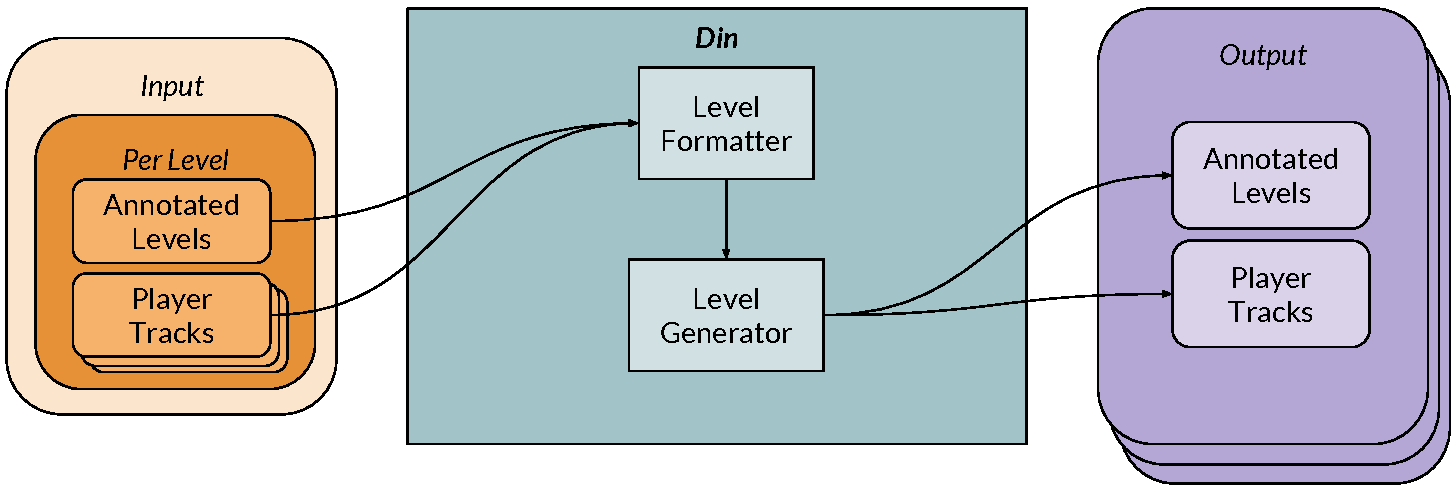
\includegraphics[width=1\textwidth]{figures/Din_Architecture.pdf}
\caption{The proposed architecture of \textit{Din}.  \textit{Din} takes in levels, player tracks, and mechanical clusters. After formatting the levels in the way that best makes sense, the formatted levels are passed to the generator which learns from the input levels.  The trained generator is capable of producing new levels (and exemplar player paths for these levels).  }
\label{fig:din_architecture}
\end{figure*}

\subsubsection{Din Architecture}

\textit{Din} is the subsystem in charge of generating levels.  It is intended that the input to \textit{Din} will be from the output of \textit{Nayru}, namely that the annotated levels and player tracks produced by \textit{Nayru} will be used by \textit{Din}; however, \textit{Din} is also intended to be generic,so as long as the level data is in the correct format, \textit{Din} should work.

As mentioned in the last section, the annotated levels ,  $\{\mathcal{L}\}$, are a set of individual levels, $\mathcal{L}$, where each level is a list of all entities (both static and dynamic) found in the level, with entities being given a unique identifier that ties their identity to the levels and mechanical clusters.  Given that the levels are just unordered lists which, while certainly a valid format to pass to many machine learning algorithms, is unlikely to be the best approach.  

Based on earlier work (see section \ref{sec:ContentGeneration}), I foresee two formats that will be utilized by \textit{Din}.

\begin{itemize}
\item 2D Tile Based --- As in the earlier Super Mario Bros. work
\item Graph Based --- As in the earlier Legend of Zelda work
\end{itemize}

\begin{figure}[ht]
\centering
    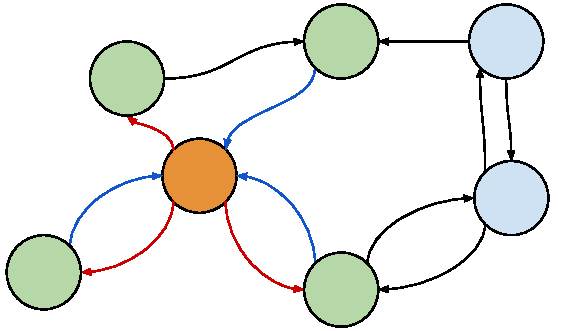
\includegraphics[width=0.97\textwidth]{figures/Din_Graph_Detail.pdf} 
   
   
    \caption{A visualization of the graph convolution process. The \textit{Orange} node is the central node of the convolution. \textit{Red} edges are outgoing, while \textit{Blue} are incoming.  The \textit{Green} nodes are the nodes in the neighborhood of the central node, while \textit{Light Blue} nodes are those that are not in the neighborhood. }
  \label{fig:convolution}
  \end{figure}
  
Levels in the 2D Tile format are $w \times h \times c+i+1$ tensors where $w$ is the width, $h$ is the height, $c$ is the number of mechanical clusters, $i$ is the number of unique entity identifiers, and the final extra dimension is a binary indicator if the player's path passed through that tile.  As in my earlier Super Mario Bros. work, \textit{Din} will use autoregressive LSTMs for learning and generation.  As in that work, \textit{Din} will use a linearized representation, but unlike that work, it is as yet unknown what format will work best for a generalized pool of games.  To that end, part of the work remaining on \textit{Din} is a generalized linearization technique.  I intend to test the following approaches:

\begin{itemize}
\item \textit{Horizontal}  --- raster left-to-right, top-to-bottom
\item \textit{Vertical}  --- raster  top-to-bottom, left-to-right
\item \textit{Majority}  --- look at the aspect ratios of the original levels and choose from either \textit{Horizontal} or \textit{Vertical} based on the most common aspect ratio (\textit{Horizontal} for levels taller than wide, \textit{Vertical} for vice versa)
\item \textit{Both}  --- encode levels both vertically and horizontally
\item \textit{Aspect}  --- For each level choose from either \textit{Horizontal} or \textit{Vertical} based on its aspect ratio (\textit{Horizontal} for levels taller than wide, \textit{Vertical} for vice versa) --- Note: \textit{Aspect} will only be considered if is different from \textit{Majority} 
\end{itemize}

Furthermore, for \textit{Aspect} and \textit{Both}, I will perform two sub-experiments, one will encode the direction  between each token in the sequence (e.g. $A \rightarrow B \rightarrow C ...$ or $A \uparrow B \uparrow C ...$) and the other will only encode the tokens.  My hypothesis is that encoding the direction will be superior to ignoring it, as ignoring it is likely to become confused with multiple directions.

The tile based levels comprise the graph format in that each individual node of the graph format is a tiled level.  Unlike the relatively straight forward training and sampling of the tile levels, graph levels have a much more complex training and sampling process.  

At training time, each node is trained in a similar manner as the above tile based manner, but instead of an autoregressive LSTM the levels are trained using a sequence-to-sequence autoencoder.  The encoder is composed of multiple layers of bidirectional LSTMs (i.e. layers with two LSTMs, one progressing forward over the node, one progressing backwards) which after the full length of the node is traversed, the final outputs are encoded into a fixed length vector.  This vector is passed to a decoder, along with a \texttt{<Go>} token, telling the decoder LSTM to start the decoding process.  At each step of decoding, the previous decoded symbol is passed to the decoder, along with the encoded state.  

After sufficient training of the individual nodes, the graphical structure is ready to be trained.  Using similar ideas to \cite{thomaskipfgraphconvolutions} and \cite{treestructuredvariationalautoencoder}, I propose a graph autoencoder.  The encoding portion of the autoencoder operates by:

\begin{enumerate}
\item Convolution --- Each node is convolved with its neighbors
\item Pooling --- After the convolutions are performed, nodes are pooled to form a coarsened graph
\end{enumerate}

  
\noindent and these steps are repeated until only a single coarsened node remains, which is then fed through a densely connected layer to a latent state.

Given a node $n$ with a set of neighbors $O$ with edge weights $e_{j\rightarrow k}$ ($1$ if the directed edge from node $j$ to $k$ exists, $0$ if it doesn't), then the convolution performs the following operation:

$c = n*w_0 + \sum_{o \in O} w_1*o*e_{n\rightarrow o}+ \sum_{o \in O} w_2*o*e_{o\rightarrow n}$

with trainable weights $w_0$ (the weight applied to the center node), $w_1$ (the weight applied to neighbors for which there is a directed edge into them), and $w_2$ (the weight applied to neighbors for which there is a directed edge out of them). A non-linear activation will be applied to $c$ (most likely a Rectified Linear Unit \cite{relu}).

The pooling stage operates by taking pairs of neighbors, finds the maximum of their values for each convolutional filter, and keeps it.  

\begin{figure}[htbp!]
\centering
    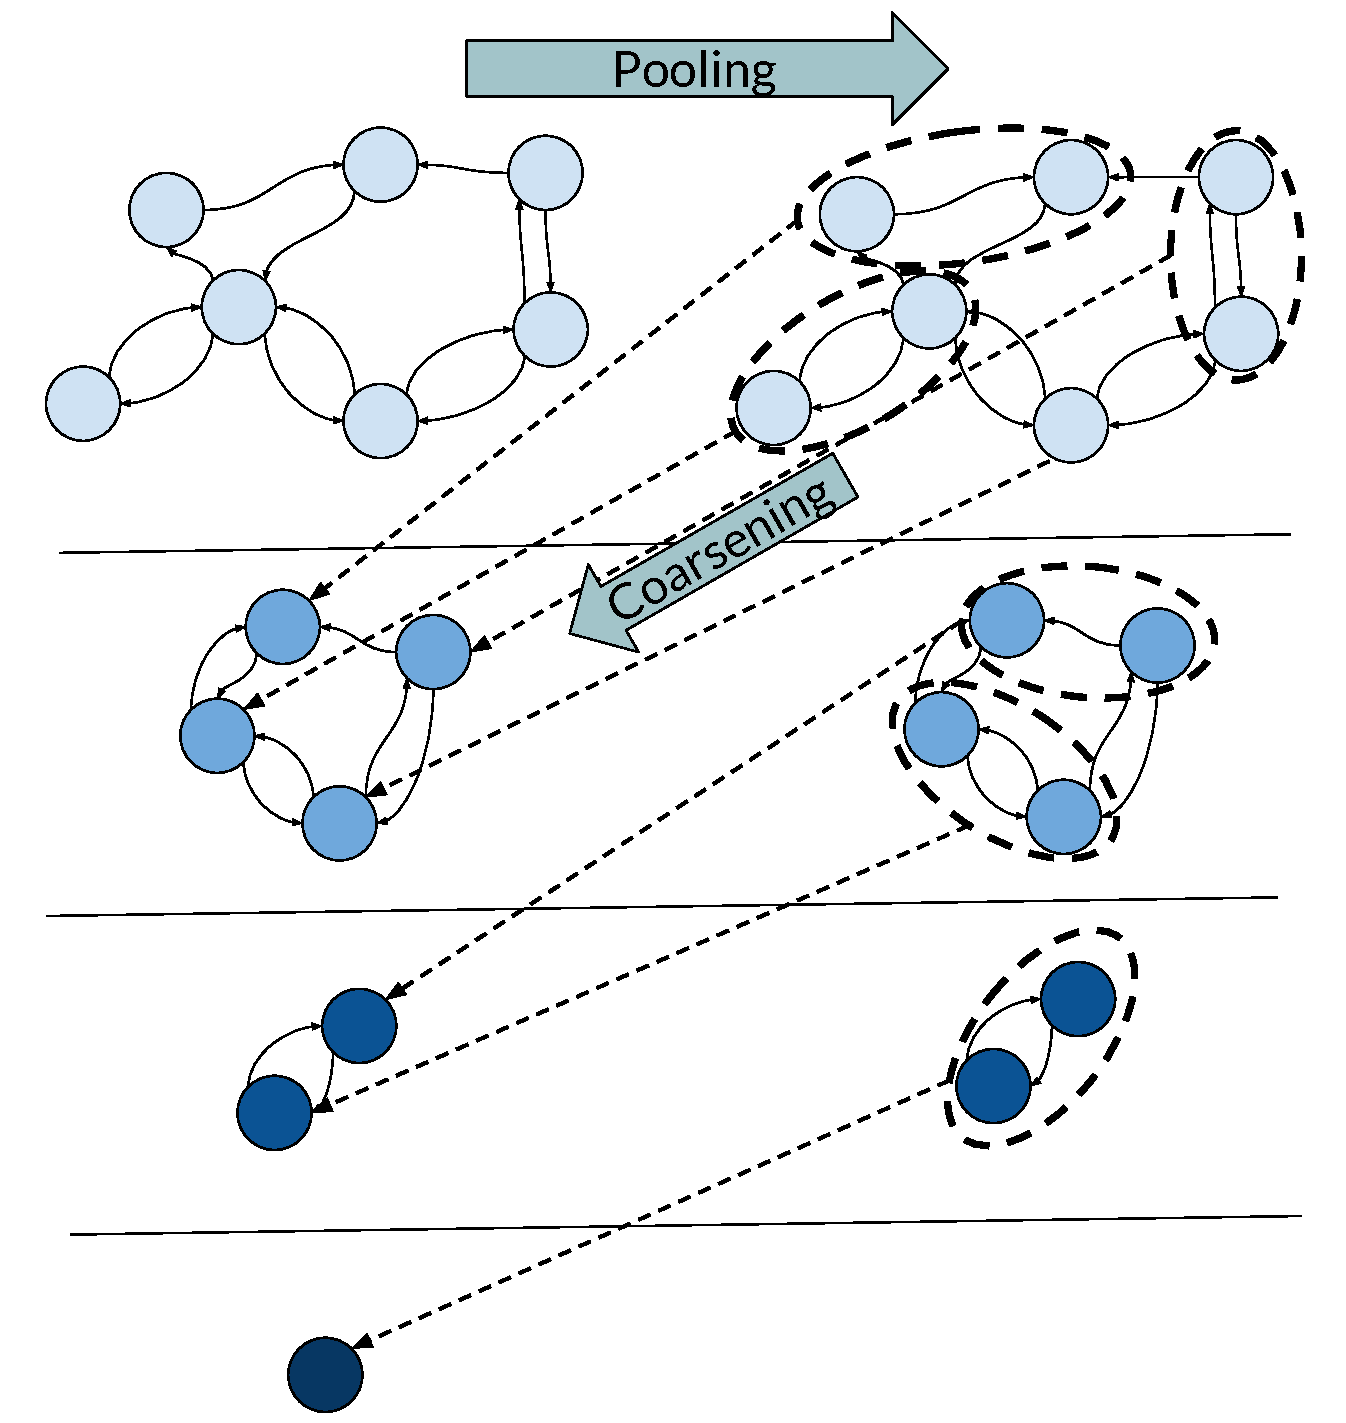
\includegraphics[width=0.97\textwidth]{figures/Pooling.pdf} 
   
   
    \caption{A visualization of the graph convolution pooling process. There are alternating pooling and coarsening phases that are iteratively applied.}
  \label{fig:pooling}
  \end{figure}
  
These steps are then repeated until a single latent state is arrived at.

There exist a number of operational questions that need to be experimented with:

\begin{itemize}
\item Should weights be shared across all levels of the graph?
\item If not, how should depth be measured? Bottom-up (e.g. leaves are depth 0) or top-down (e.g. the final source node is depth 0)? 
\item If it is bottom up, how should conflicting depths be handled? Minimum or maximum?
\end{itemize}

The decoding process is a bit more involved.  Given a latent representation $z$ we need the following functions:

\begin{itemize}
\item \textsc{Is\_Terminal}$(z)$ -- a logistic function that specifies whether the given node should be a terminal node
\item \textsc{Get\_Children}$(z)$ -- a function from the $k$ dimensional latent space that produces two $k$ dimensional vectors, the children of the node, used only if the node is non-terminal
\item \textsc{Reify}$(z)$ --- a function from the $k$ dimensional graph latent space to the $h$ dimensional tile latent space, used if the node is terminal

\item \textsc{Find\_Links}$(T)$ --- a function from a binary tree structured graph that returns the links between nodes.  The output is a sequence of leaf id pairs signifying an edge from the first leaf to the second. 
\end{itemize}

Given that, decoding operates via decoding the root level latent node with the following procedure:


\begin{algorithmic}[1]
\Procedure{Decode}{$z$}
\If {\textsc{Is\_Terminal}$(z)$}
\State \Return \textsc{Reify}$(z)$
\Else 
\State $z_{l}, z_{r} \gets $  \textsc{Get\_Children}$(z)$
\State \Return $\langle$ Decode($z_l$) ,  Decode($z_r$) $\rangle$ 
\EndIf
\EndProcedure
\end{algorithmic}

This returns a binary tree form of the graph, where each leaf represents an actual node of the graph.   \textsc{Find\_Links} is then applied to the tree, returning the links.

Given that there are many possible trees that describe the graph coarsening \cite{Comparisonofcoarseningschemesformultilevelgraphpartitioning}, I intend to utilize domain knowledge to choose the order of coarsening.  Given that the graphs come from play throughs, I will order the nodes in the order that they are capable of being reached by the player.  Then when the pooling step occurs, the lowest neighbor will be chosen.



\subsubsection{Work Remaining}

The graph learning/generation portion represents the largest portion remaining 

\subsection{Farore --- Game Behavior Generation}
\begin{quotation}
\textit{Farore's rich soul created all life forms who would uphold the law.}  \\ \indent \indent --- Ocarina of Time
\end{quotation}

\bibliographystyle{apalike-oadoi}
\bibliography{sample}

\end{document}

\bibliographystyle{apalike-oadoi}
\bibliography{sample}

\end{document}
